%%%% CAPÍTULO 4 - RESULTADOS E DISCUSSÃO

\chapter{Resultados}
\label{cap:resultados}

Trata-se de um sistema complexo que foi modelado levando em consideração aspectos reais da utilização de software em cenários de uso reais. O projeto foi desenvolvido de forma consistente e replicável, seguindo as boas práticas de desenvolvimento de software e utilizando tecnologias modernas e de mercado.

O principal resultado deste trabalho é um artefato completo e funcional que pode ser utilizado pela \gls{utfpr} para gerenciar instâncias de máquinas virtuais na \gls{aws} de forma segura e eficiente, bem como replicado e configurado para diferentes instituições de ensino com interesse em utilizar sistemas de \gls{vdi} em nuvem pública para fins acadêmicos.

A demonstração completa dos resultados obtidos nesse trabalho se da através da apresentação do sistema em funcionamento pelo ponto de vista do usuário final. Sistema este que foi implementado e testado para satisfazer os requisitos e princípios de modelagem definidos na \autoref{sec:modelagemDoSistema}. Além disso será apresentada uma estimativa de custos para a utilização do sistema em diferentes cenários de uso.

\section{O sistema em funcionamento}
\label{sec:oSistemaEmFuncionamento}

Ao acessar o cliente \textit{web} através de um navegador pela primeira vez o usuário é redirecionado para a página de autenticação, como apresentado na \autoref{fig:signInPage}. Nesse momento ele pode inserir suas credencias de acesso se já possuir uma conta criada, ou acionar o botão com o título: \texttt{Entrar com a UTFPR}, que o redireciona para a página de autenticação do provedor de identidade externo da \gls{utfpr}. Há também a opção de redefinir senha, que oferece um método de recuperação de conta para usuários cadastrados diretamente do sistema.



\begin{figure}[H]
%\captionsetup{width=0.55\textwidth}%% Largura da legenda
\caption{Página de Autenticação}
\label{fig:signInPage}
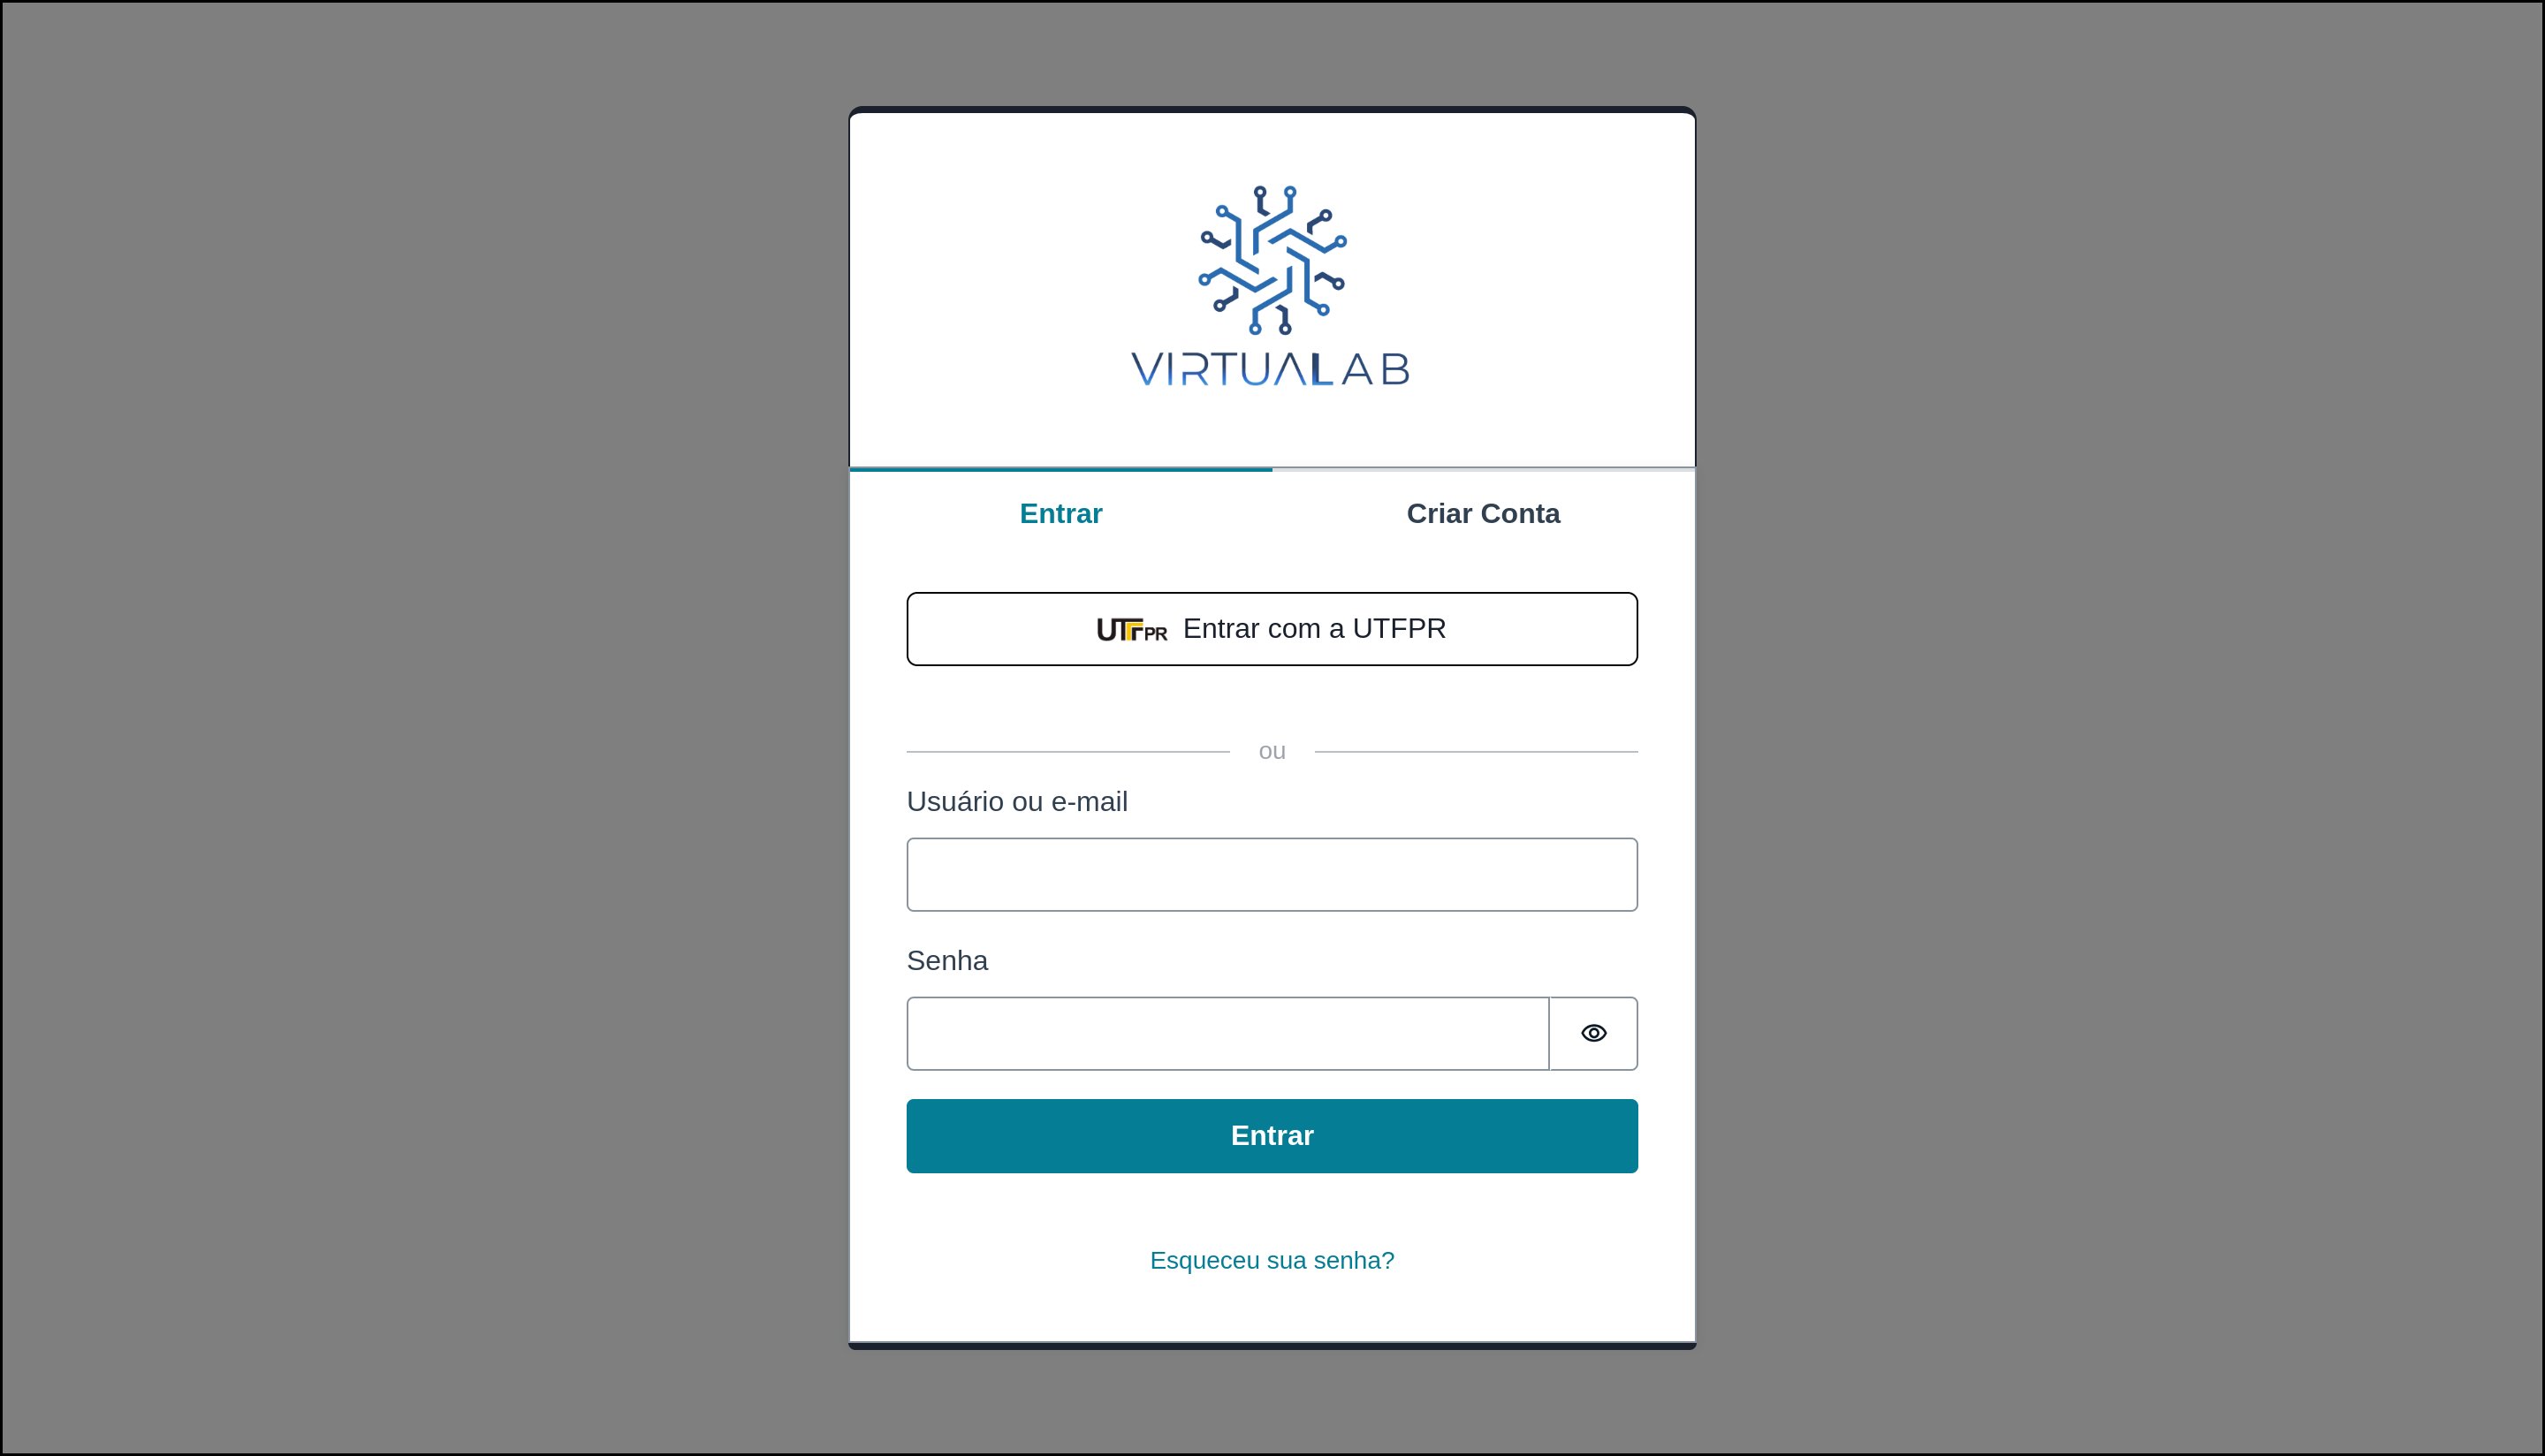
\includegraphics[width=\textwidth]{capitulos/3-resultados/files/sign-in.png}
\fonte{Autoria Própria (2024)}
\end{figure}

No caso onde o usuário não possui uma conta cadastrada e nem credencias de acesso para utilizar o login integrado com a \gls{utfpr}, ele deve seguir para a página de cadastro de uma nova conta, como apresentado na \autoref{fig:signUpPage}. Nessa página o usuário deve preencher os campos obrigatórios e acionar o botão \texttt{Criar Conta}  para que a conta seja criada.

Mesmo podendo se autenticar com uma conta criada manualmente, ao usuário será atribuído o cargo de \gls{upen}, que não o permite interagir com os recursos do sistema.

Caso essa página não seja adequada para o ambiente de produção, ela pode ser desativada através das configuração de implantação do sistema. Isso vale também para o botão de integração com o provedor de identidade externo. Porém se as duas funcionalidades forem desabilitadas o sistema só permitirá a criação de usuários através da interface do serviço \textit{AWS Cognito} no painel de administração da \gls{aws}.


\begin{figure}[H]
%\captionsetup{width=0.55\textwidth}%% Largura da legenda
\caption{Página de Cadastro}
\label{fig:signUpPage}
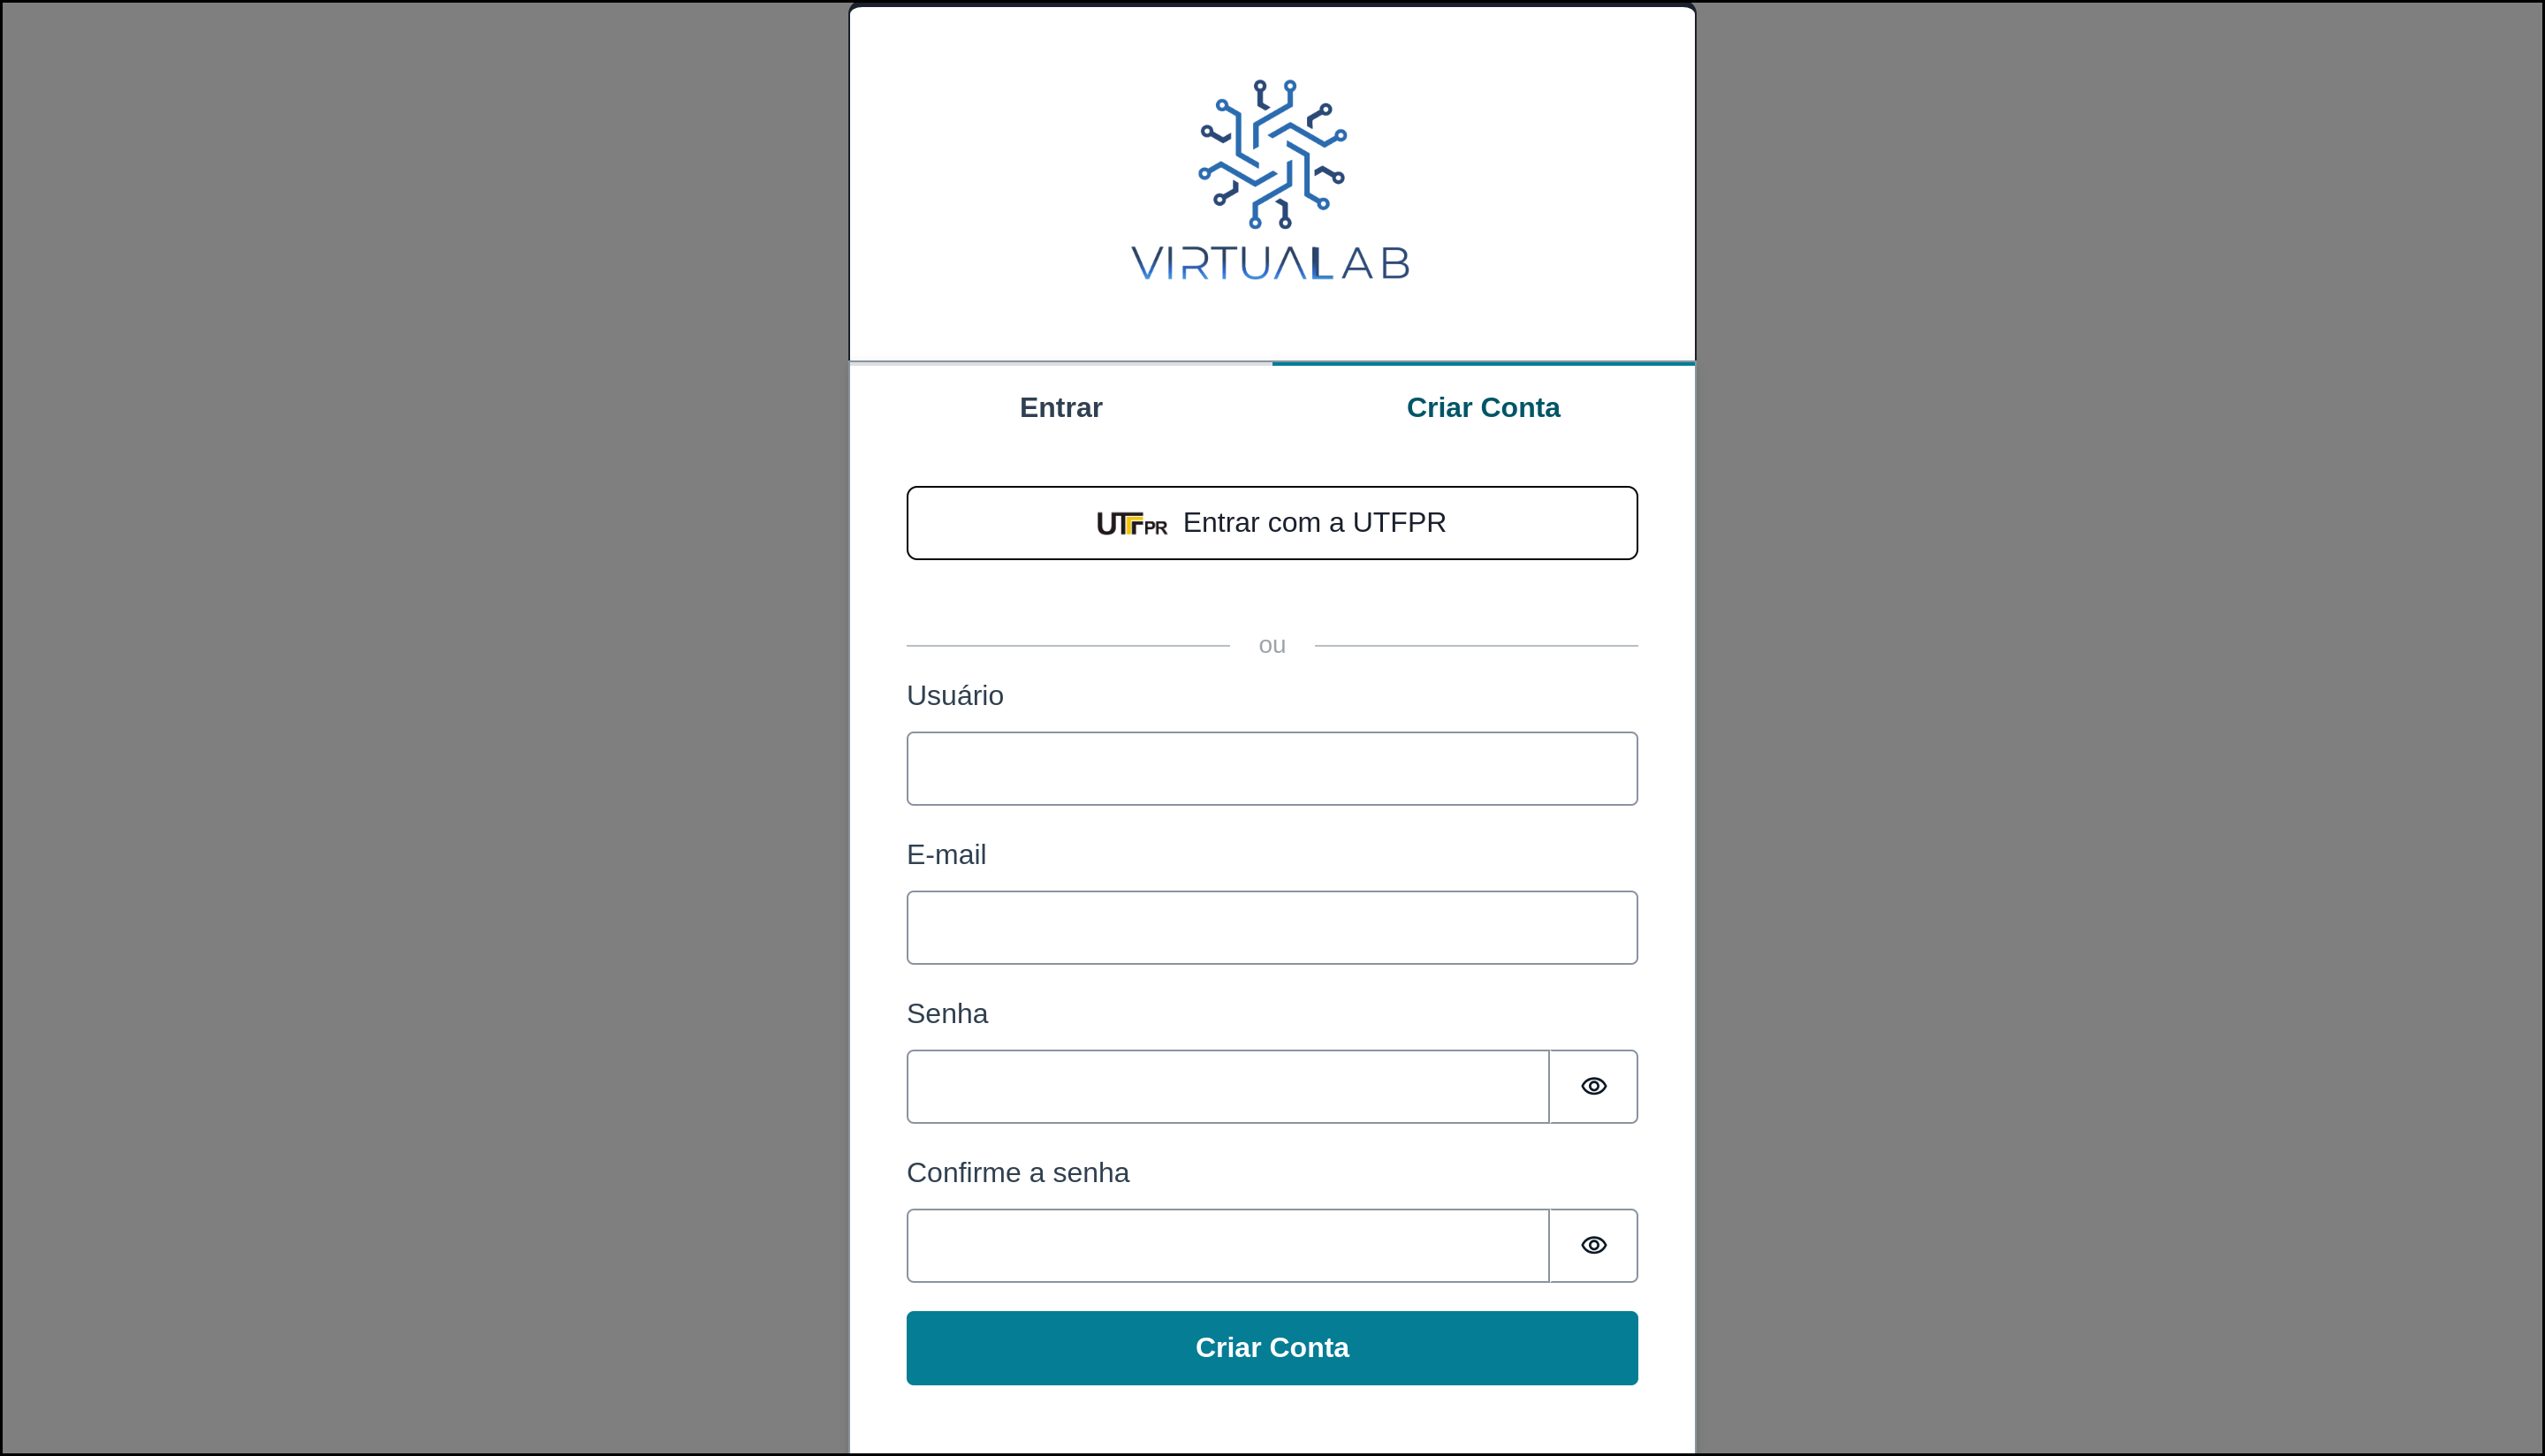
\includegraphics[width=\textwidth]{capitulos/3-resultados/files/sign-up.png}
\fonte{Autoria Própria (2024)}
\end{figure}

Caso o usuário receba acesso completo ao sistema, a página inicial do cliente web será a listagem das instâncias tanto para \glspl{ucom} e \glspl{uadm}, como apresentado na \autoref{fig:instancesPage}.

Nessa página o usuário pode visualizar todas as instâncias que ele possui acesso, bem como realizar as operações de gerenciamento das mesmas.

Caso a instância esteja ligada, o usuário pode desligá-la, reiniciá-la ou acessá-la através dos botões \texttt{Desligar}, \texttt{Reiniciar} e \texttt{Acessar}. Caso a instância esteja desligada, o usuário pode ligá-la ou deletá-la através dos botões \texttt{Ligar} e \texttt{Excluir} respectivamente. 

Ainda nessa página o usuário pode aplicar filtros de busca para encontrar instâncias específicas ordenar as instâncias por diferentes critérios e criar novas instâncias através do botão \texttt{Nova Instância}, no canto superior direito da tela.

\begin{figure}[H]
%\captionsetup{width=0.55\textwidth}%% Largura da legenda
\caption{Página de listagem de instâncias}
\label{fig:instancesPage}
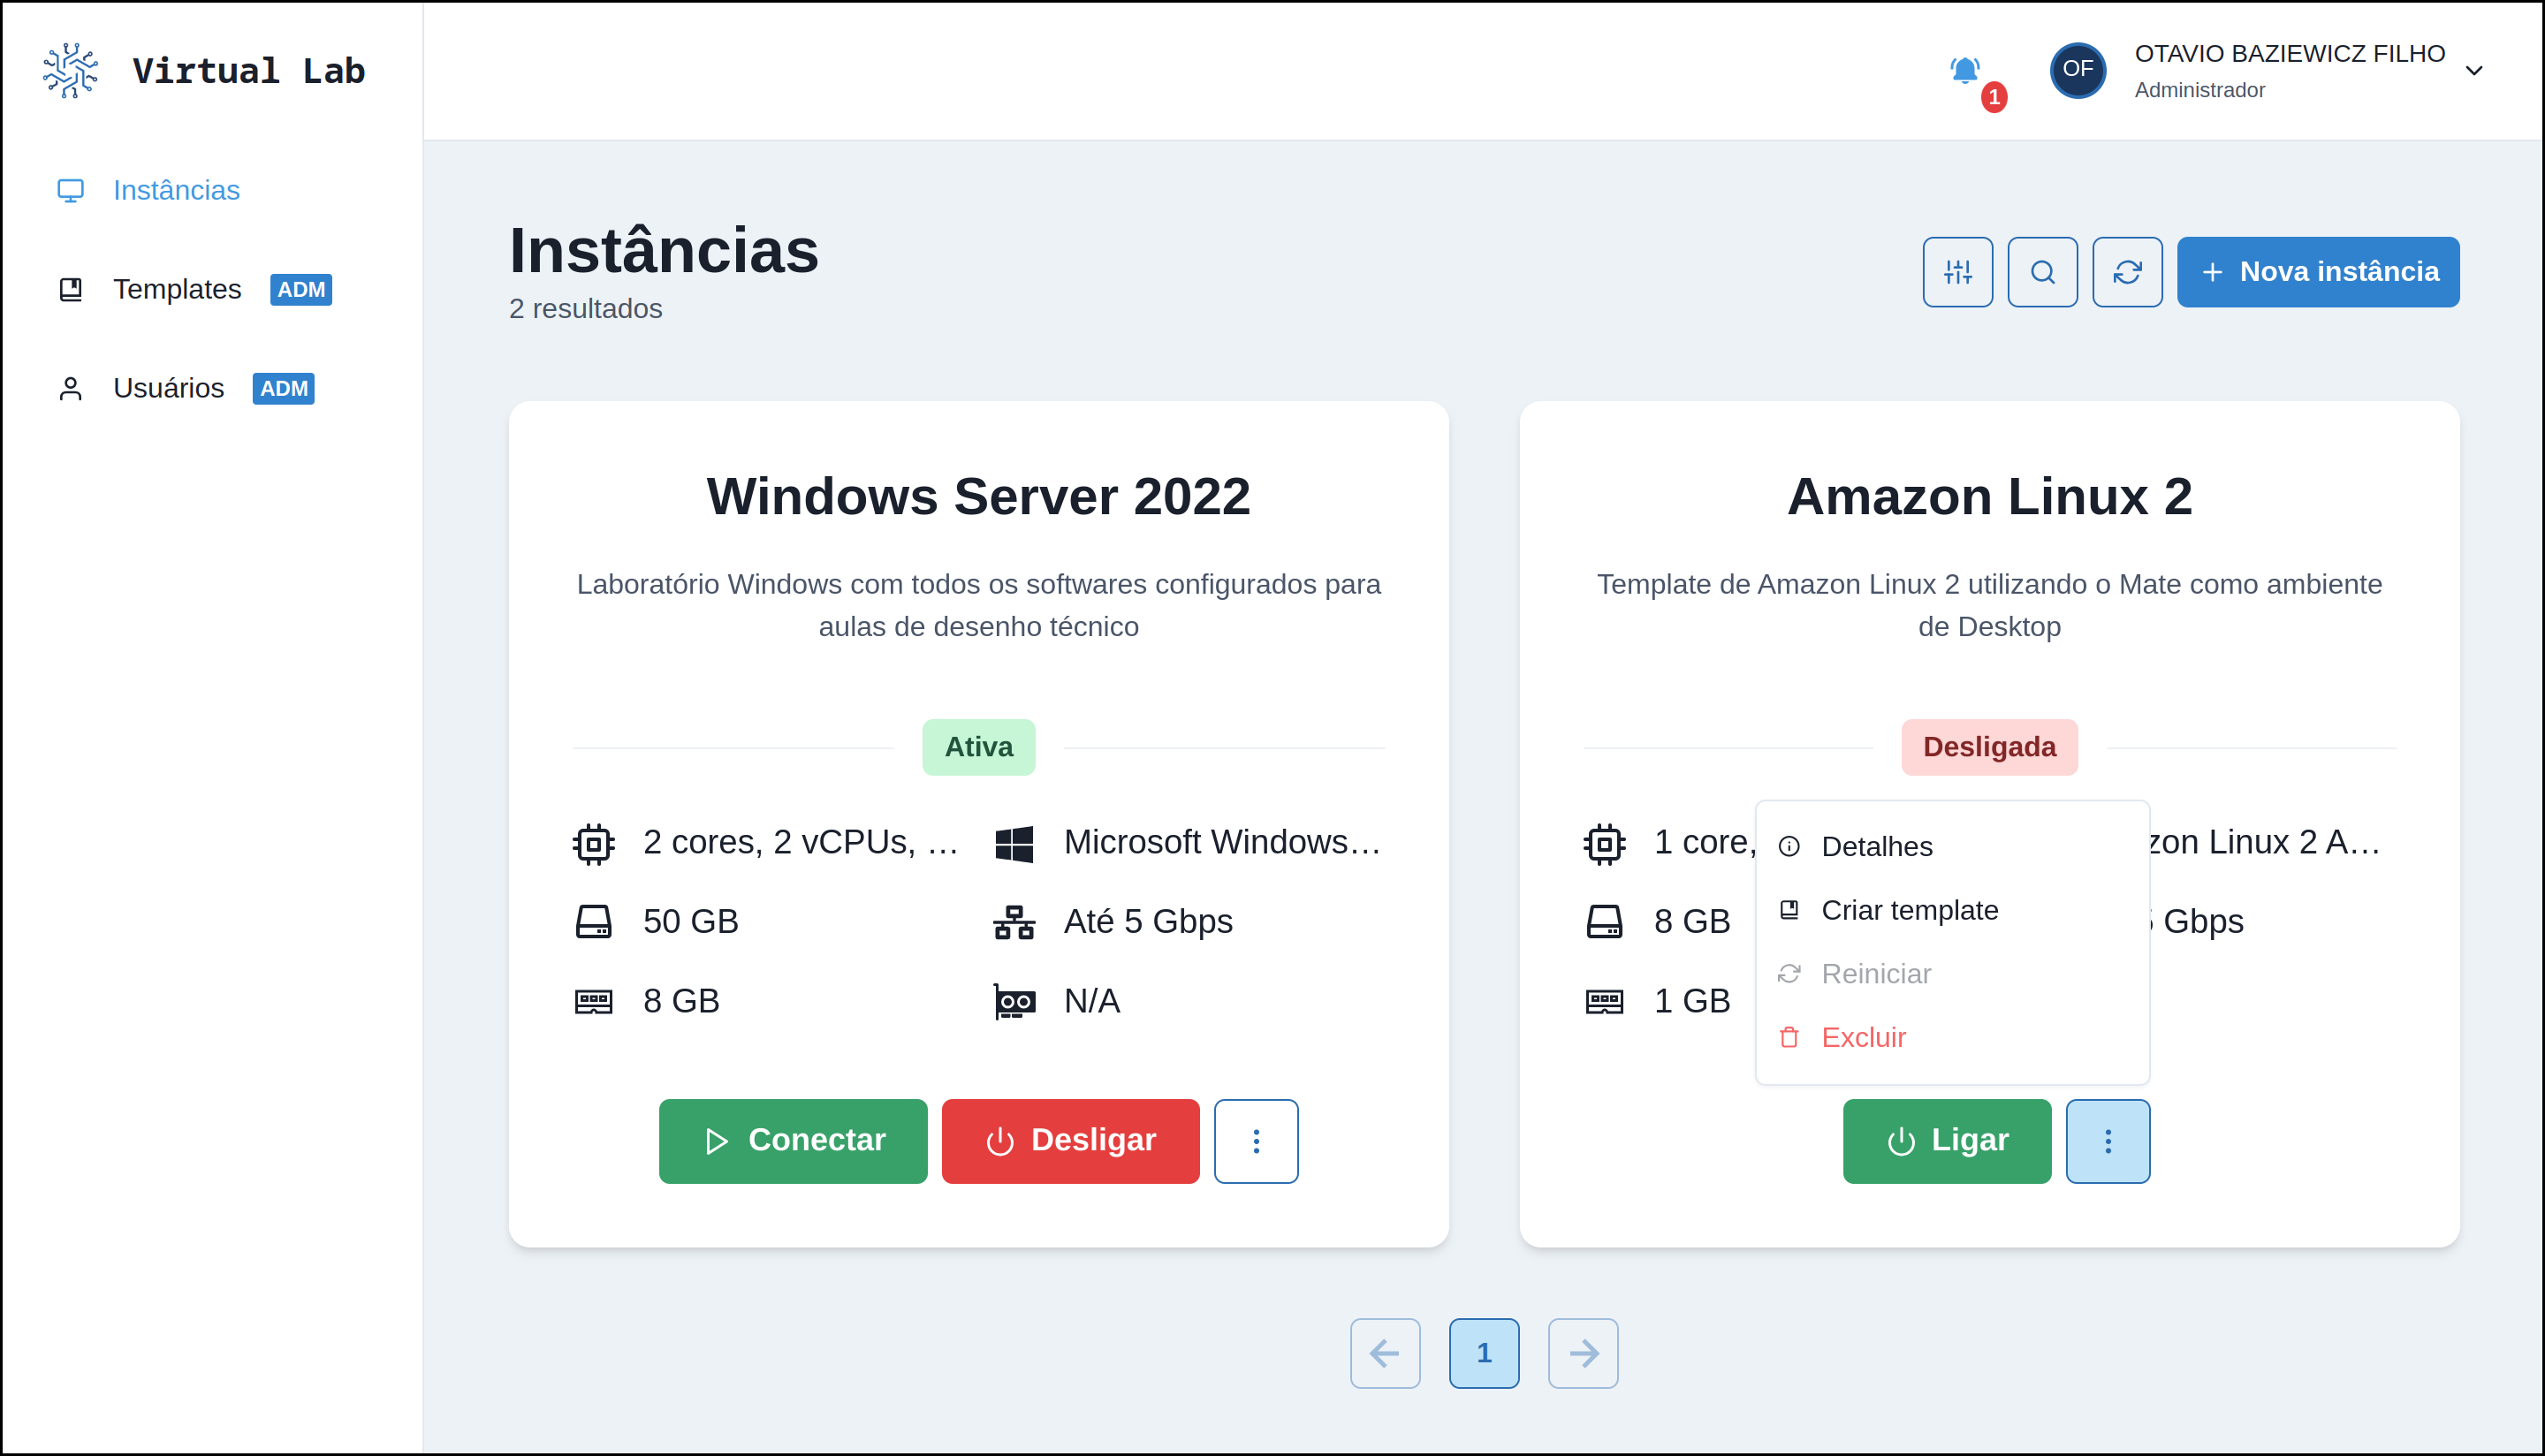
\includegraphics[width=\textwidth]{capitulos/3-resultados/files/instances.png}
\fonte{Autoria Própria (2024)}
\end{figure}

Todos os detalhes de uma instância podem ser visualizados através do botão \texttt{Detalhes}, que apresenta ao usuário o modal de detalhes da instância, como pode ser visto na \autoref{fig:instanceDetails}. Essas informações não são editáveis, mas permitem que o usuário tenha conhecimento de todos os detalhes da instância de maneira agrupada.

\begin{figure}[H]
%\captionsetup{width=0.55\textwidth}%% Largura da legenda
\caption{Modal de detalhes de uma instância}
\label{fig:instanceDetails}
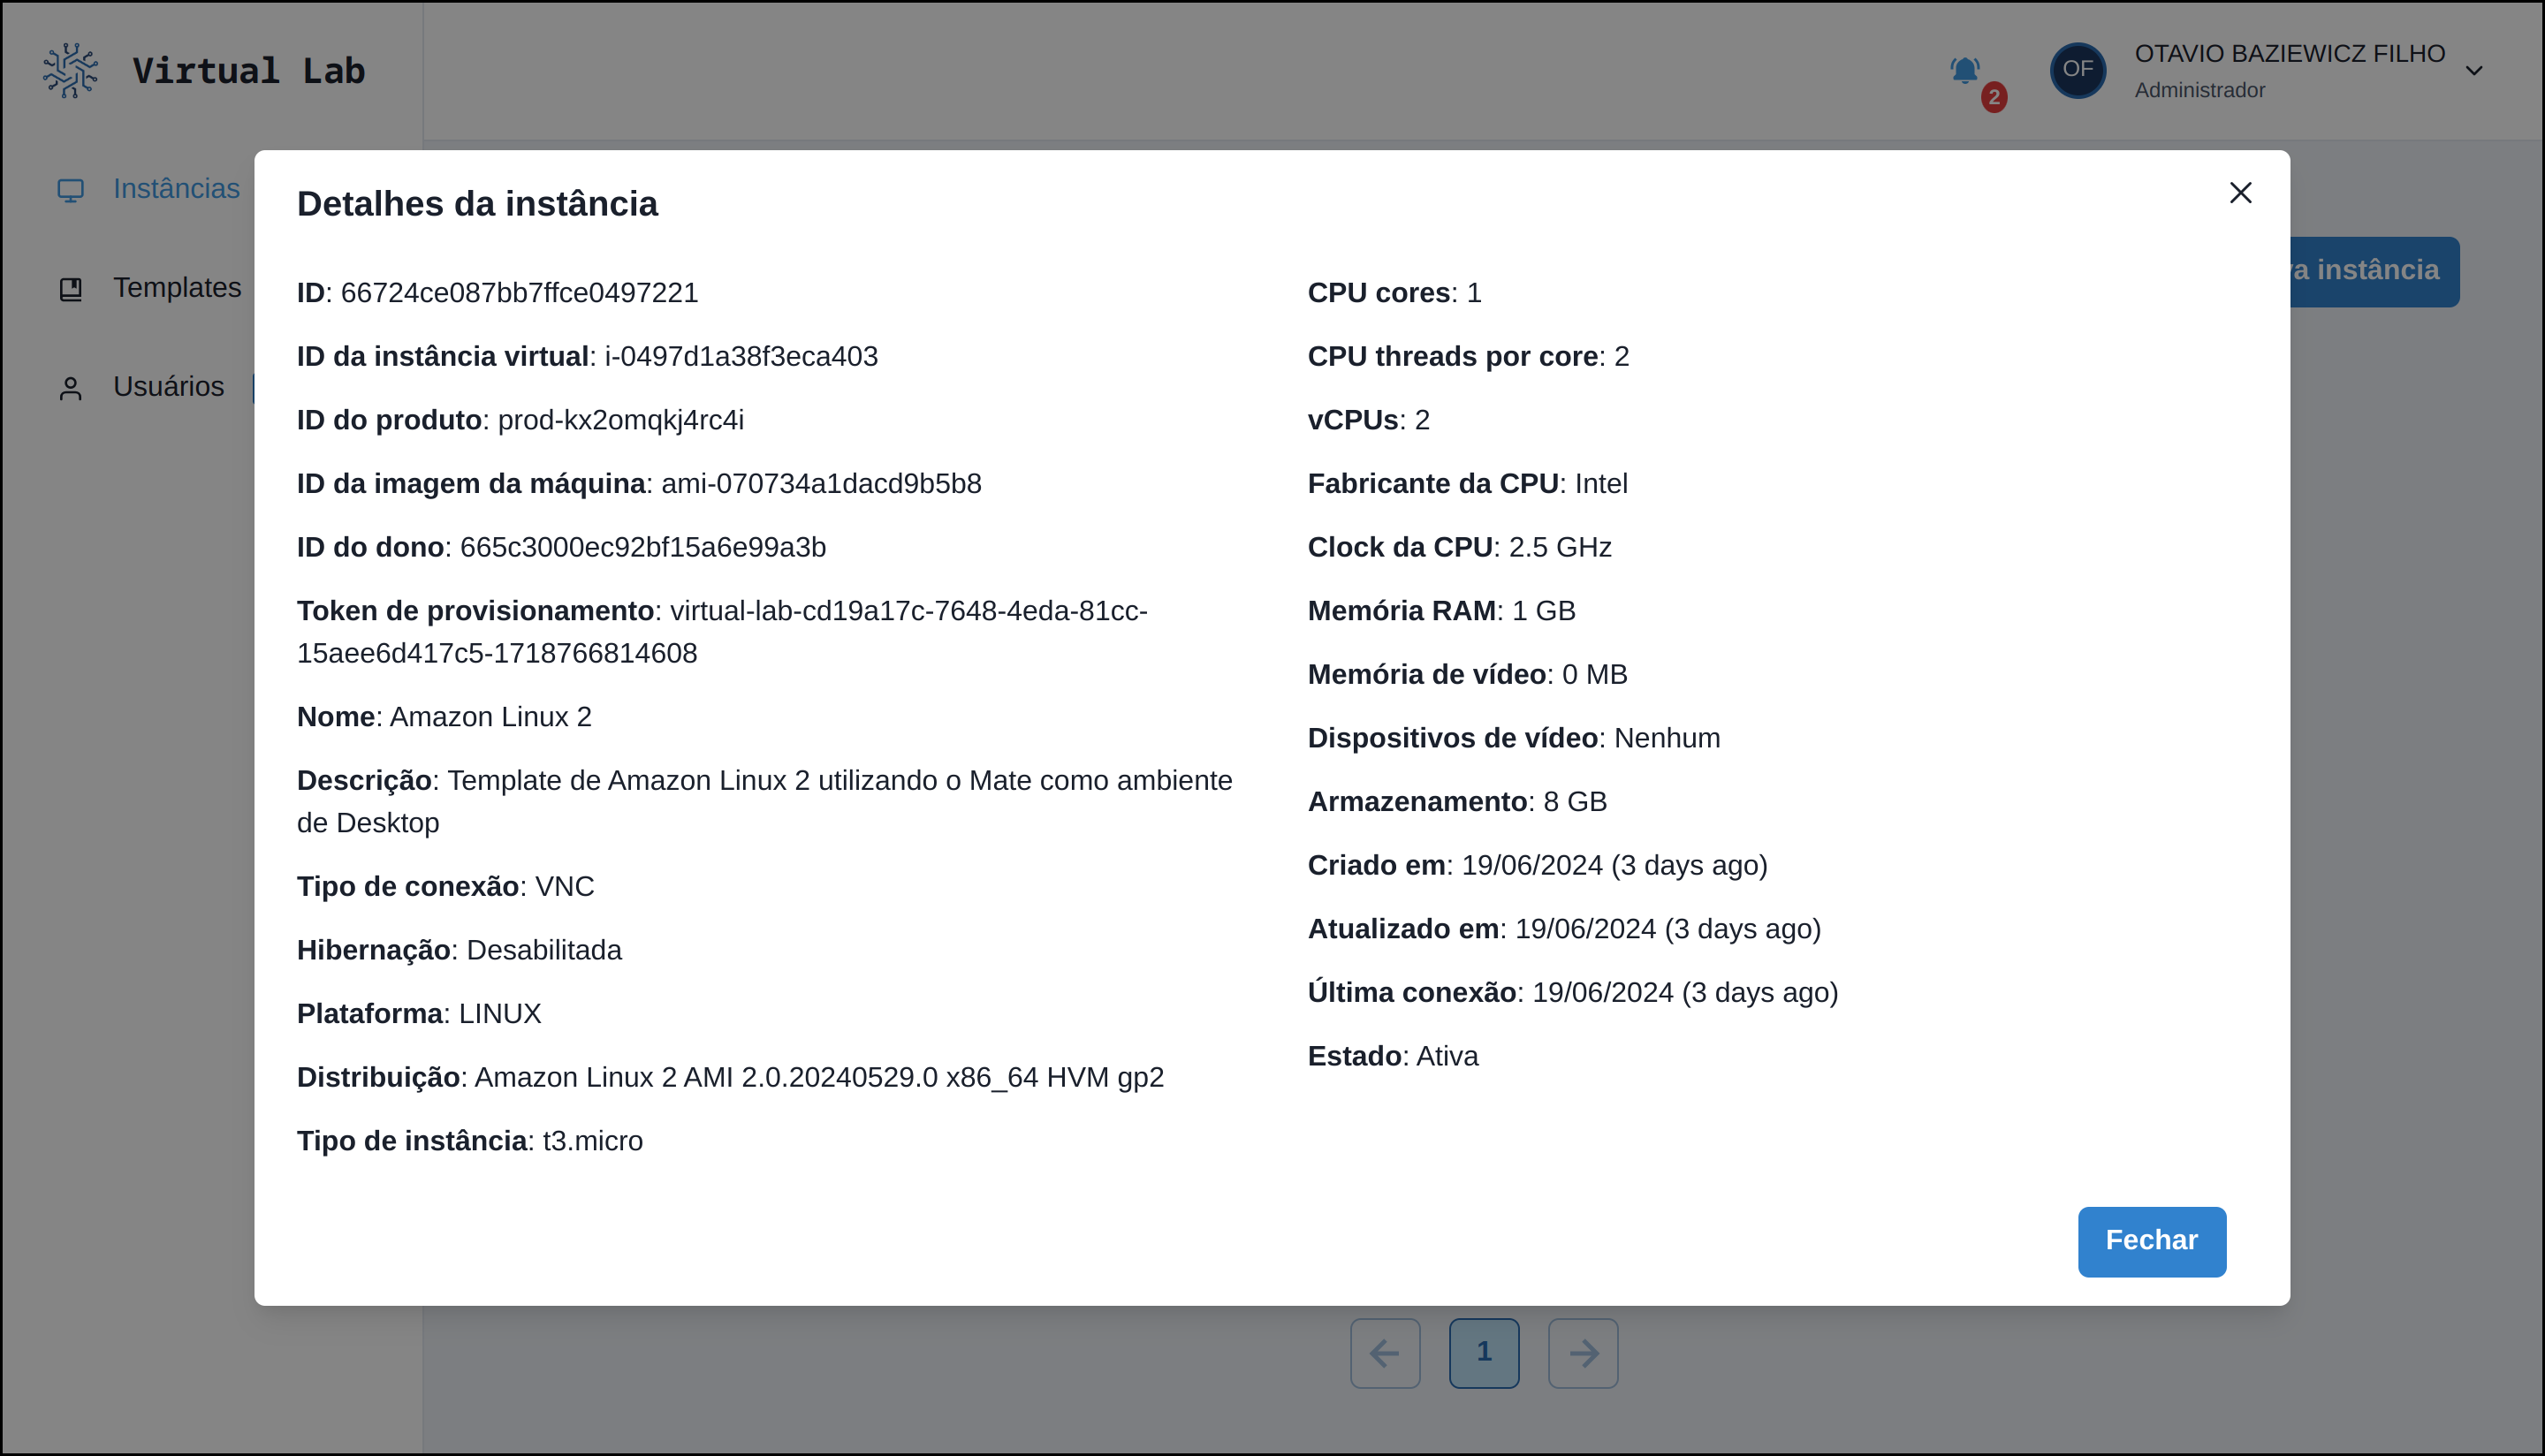
\includegraphics[width=\textwidth]{capitulos/3-resultados/files/instance-details.png}
\fonte{Autoria Própria (2024)}
\end{figure}

Para usuários com o cargo de \gls{uadm} há ainda a opção de de criar um template de instância a partir de uma instância existente, através do botão \texttt{Criar Template}. Ao acionar esse botão, o usuário deve preencher os campos obrigatórios na página de criação de template, como apresentado na \autoref{fig:createTemplateFromInstance}, e então acionar o botão \texttt{Criar Template} para confirmar a criação. Nesse momento, o sistema faz uma cópia da instância selecionada e a transforma em um template através de um processo que pode levar alguns minutos, dependendo da quantidade de dados a serem copiados e da quantidade de armazenamento selecionada para o template.

\begin{figure}[H]
%\captionsetup{width=0.55\textwidth}%% Largura da legenda
\caption{Modal de criação de template a partir de uma instância existente}
\label{fig:createTemplateFromInstance}
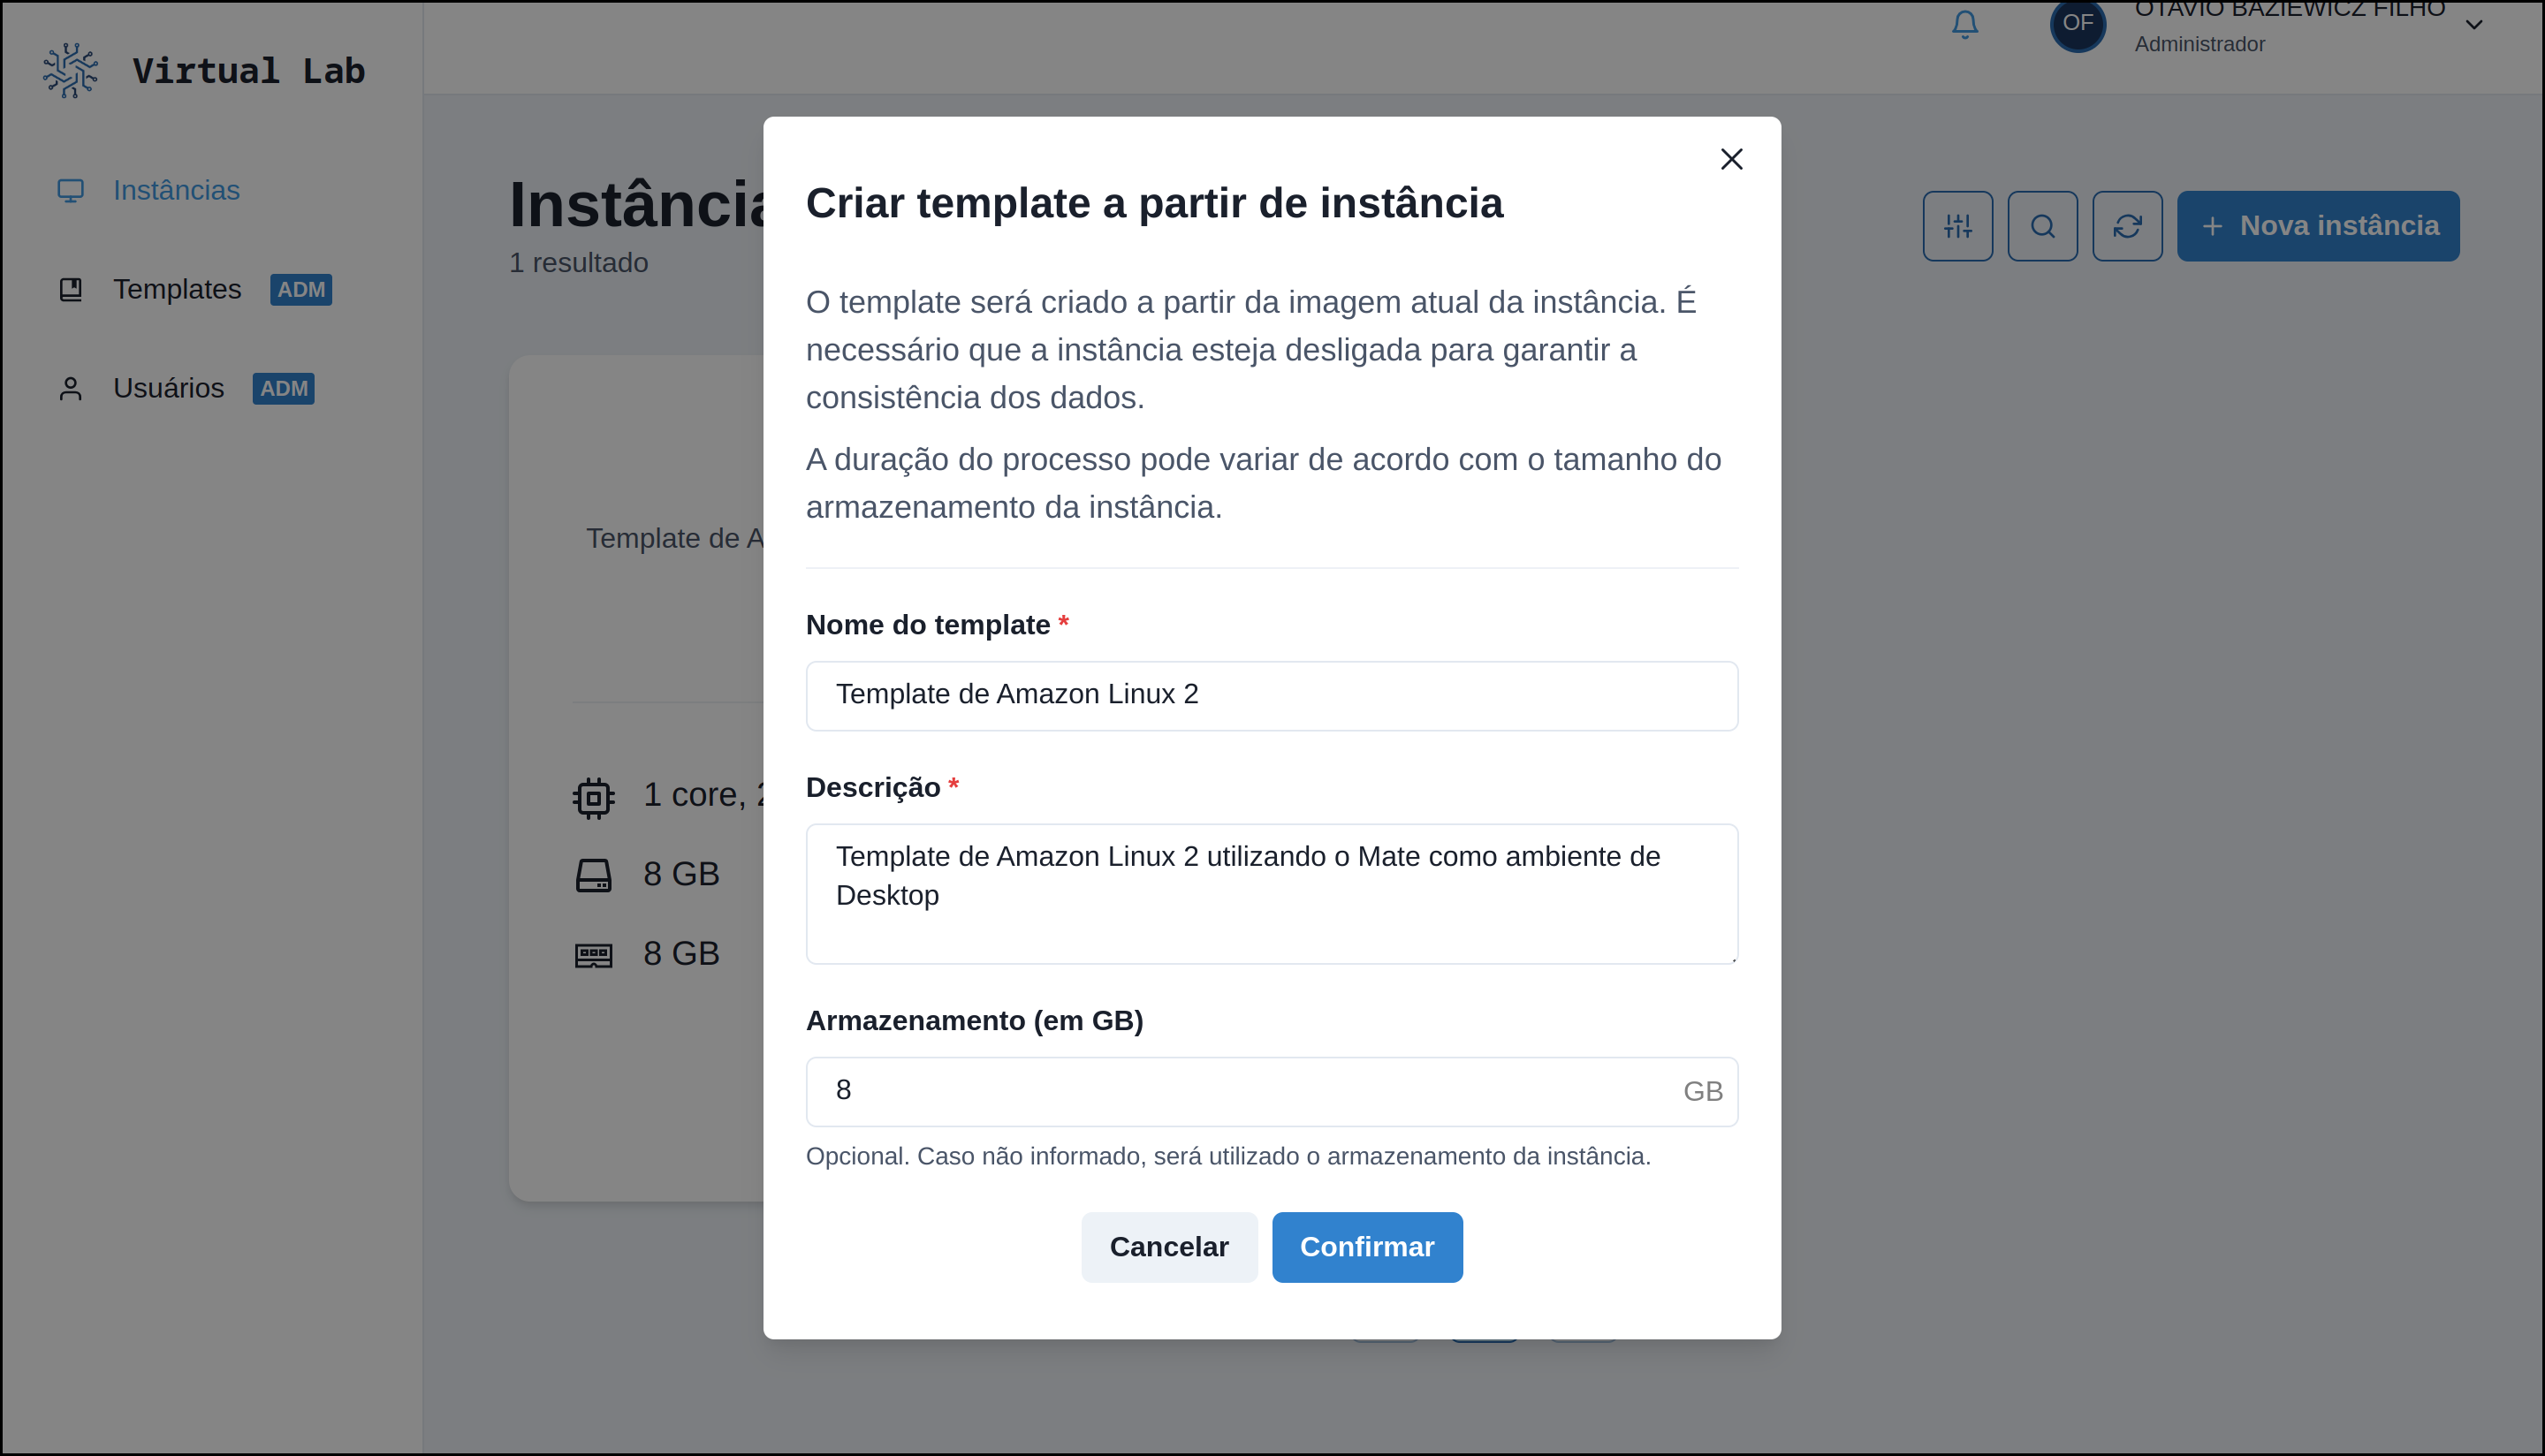
\includegraphics[width=\textwidth]{capitulos/3-resultados/files/create-template-from-instance.png}
\fonte{Autoria Própria (2024)}
\end{figure}

Se o usuário optar por criar uma nova instância através do botão \texttt{Nova Instância}, ele será redirecionado para a página onde todos os templates de instâncias disponíveis são listados, como apresentado na \autoref{fig:availableTemplatesPage}. Nessa página o usuário pode selecionar um template escolhido e acionar o botão \texttt{Criar a partir deste template}, que apresenta o modal de especificação dos parâmetros de criação da instância, como mostra a \autoref{fig:createInstance}.

\begin{figure}[H]
%\captionsetup{width=0.55\textwidth}%% Largura da legenda
\caption{Página de listagem dos templates de instâncias disponíveis para criação de uma nova instância}
\label{fig:availableTemplatesPage}
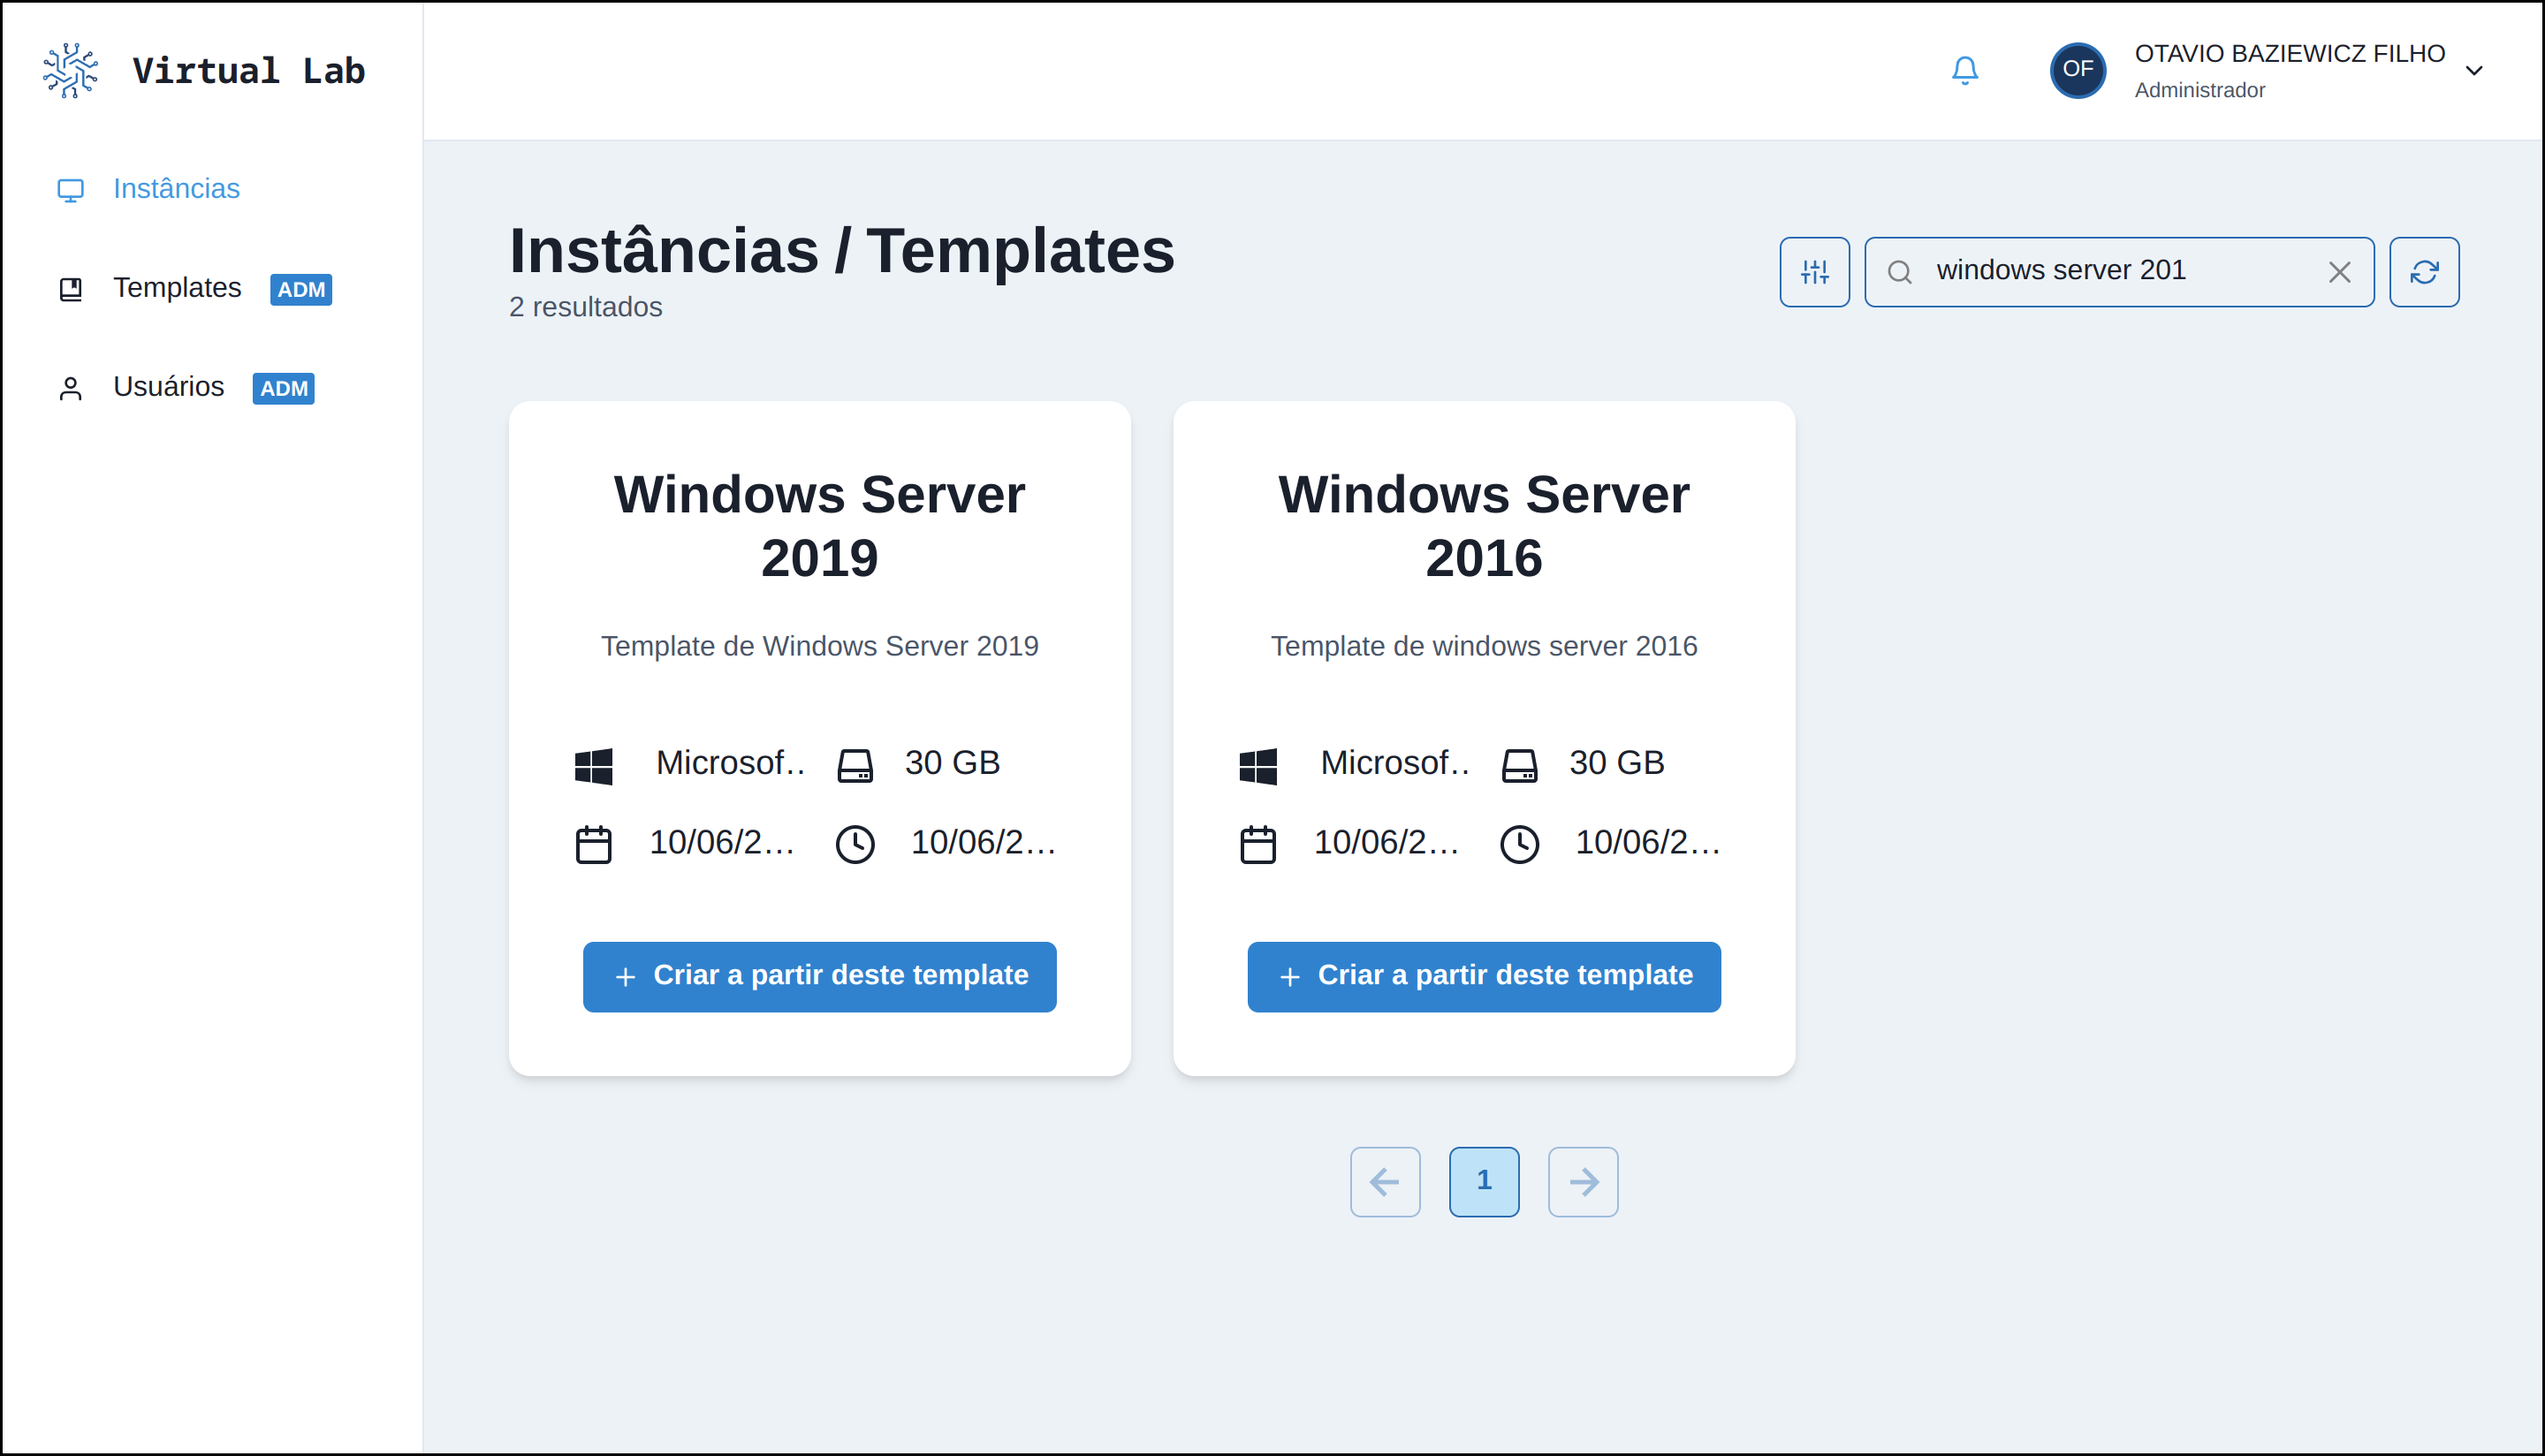
\includegraphics[width=\textwidth]{capitulos/3-resultados/files/available-templates.png}
\fonte{Autoria Própria (2024)}
\end{figure}

Na página de especificação dos parâmetros para a criação de uma nova instância, o usuário tem a opção de atribuir um nome e uma descrição para a instância, bem como escolher o tipo de hardware da instância e se o recurso de hibernação será habilitado. A lista de tipos de hardware disponíveis é dinâmica e é carregada a partir da aplicação de API, onde são mostrados todas opções previamente atribuídas pelo administrador do sistema. Para iniciar o processo de criação o usuário pode acionar o botão \texttt{Criar Instância} que entra em modo de carregamento e em seguia redireciona o usuário para a listagem de instâncias, apresentada pela \autoref{fig:instancesPage}.


\begin{figure}[H]
%\captionsetup{width=0.55\textwidth}%% Largura da legenda
\caption{Modal de criação de uma nova instância}
\label{fig:createInstance}
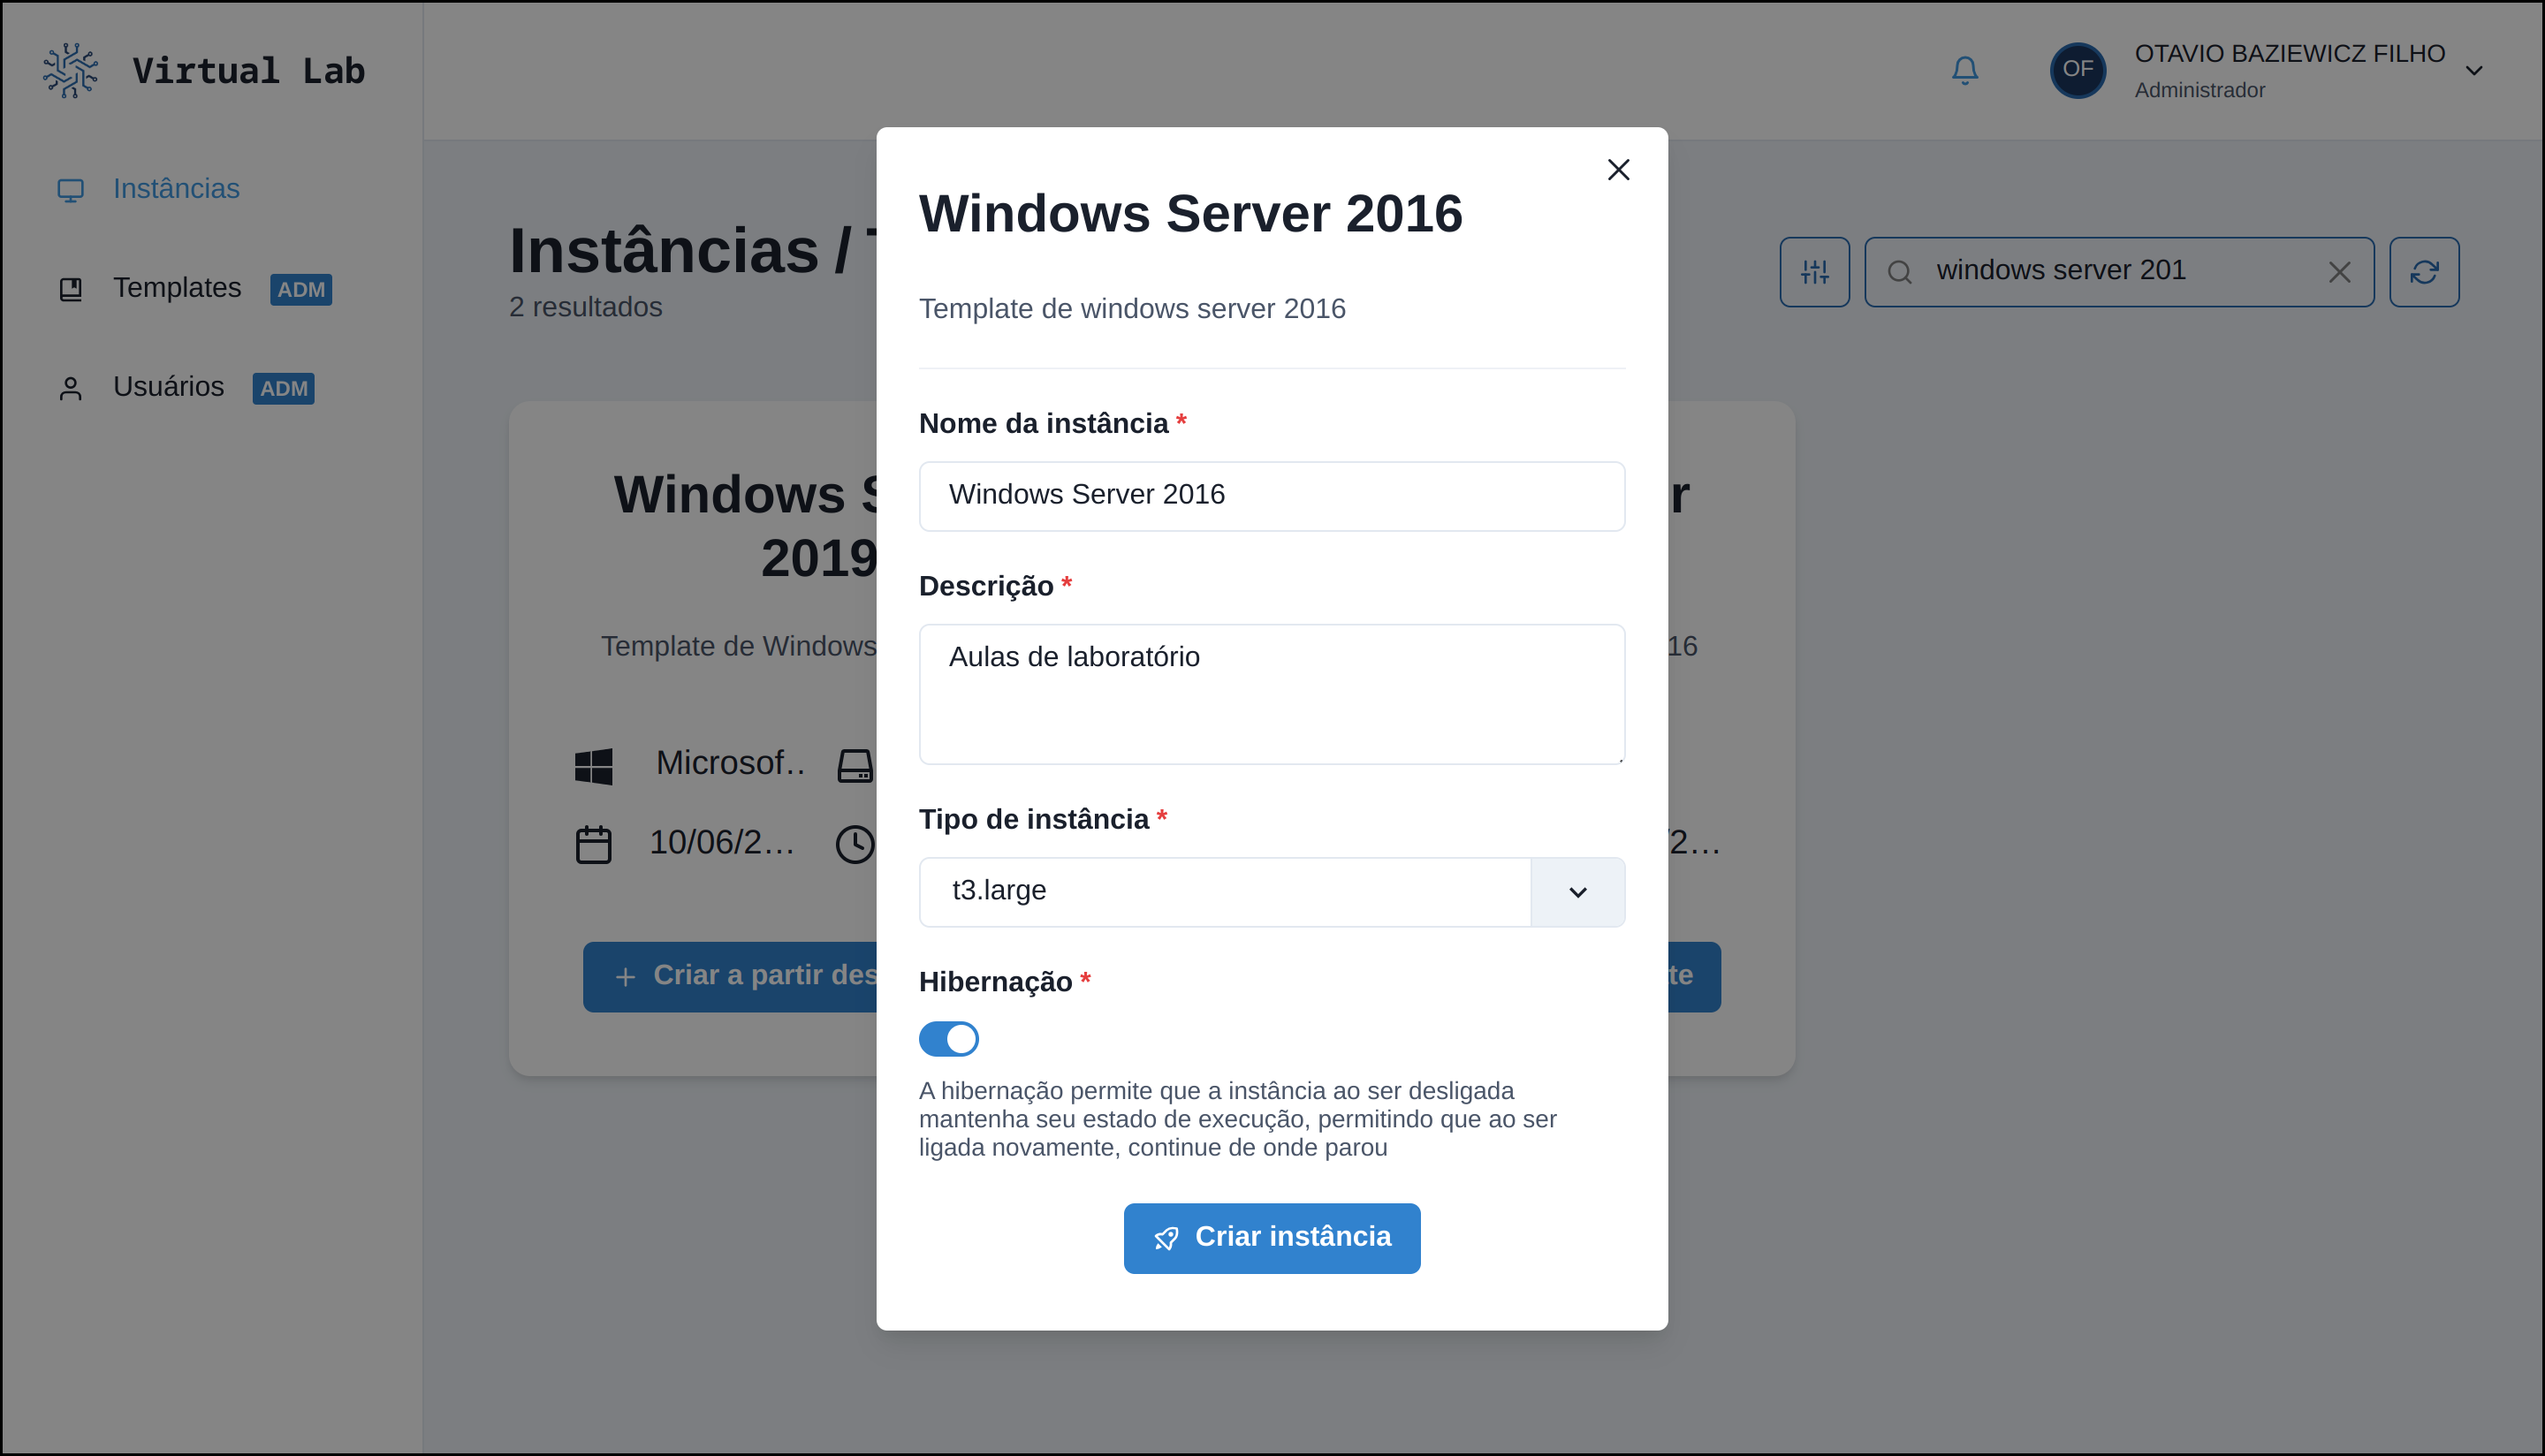
\includegraphics[width=\textwidth]{capitulos/3-resultados/files/create-instance.png}
\fonte{Autoria Própria (2024)}
\end{figure}

Enquanto a instância estiver sendo criada o usuário recebe notificações em tempo real sobre o andamento do processo, como apresentado na \autoref{fig:notificationsComponent}. Essas notificações são exibidas em através de um botão com símbolo de sino que é fixado no canto inferior direito da tela e permite que o usuário marque as notificações como lidas ou as exclua.

\begin{figure}[H]
%\captionsetup{width=0.55\textwidth}%% Largura da legenda
\caption{Componente de notificações}
\label{fig:notificationsComponent}
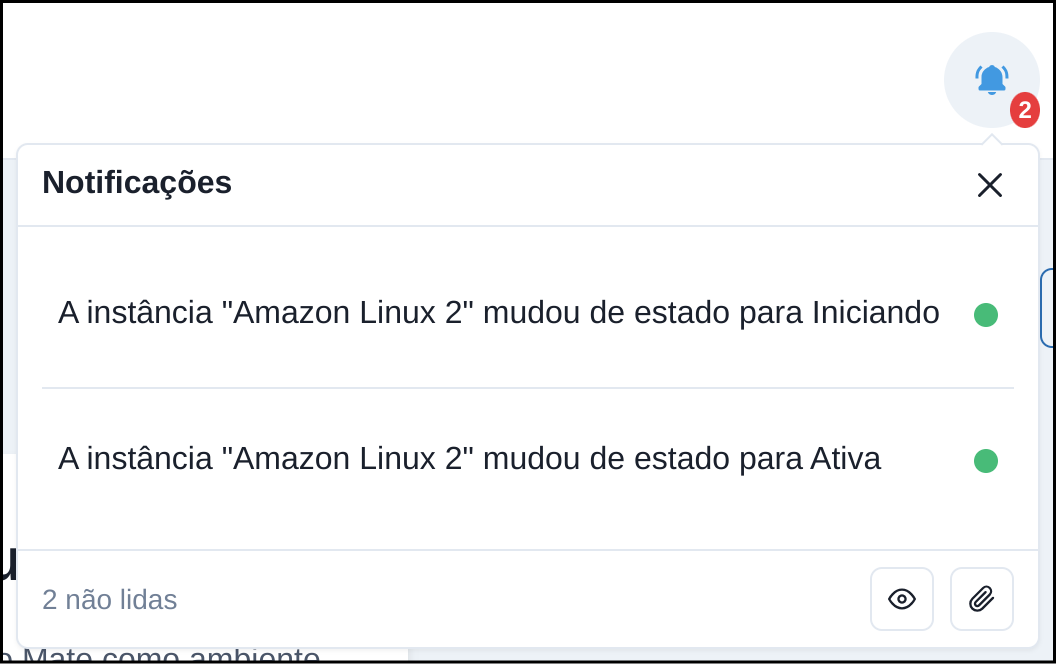
\includegraphics[width=\textwidth]{capitulos/3-resultados/files/notifications.png}
\fonte{Autoria Própria (2024)}
\end{figure}

Quando o processo de configuração da instância é concluído, o usuário pode iniciar uma conexão através do botão \texttt{Conectar} mostrado na \autoref{fig:instancesPage}. Ao acionar esse botão o usuário é redirecionado para a página de conexão, onde o usuário tem acesso à interface remota da instância, como apresentado na \autoref{fig:connectionPage}. Nessa página o usuário pode interagir com a instância e também voltar para a listagem de instâncias através do botão \texttt{Encerrar sessão}.

\begin{figure}[H]
%\captionsetup{width=0.55\textwidth}%% Largura da legenda
\caption{Página de conexão com instância}
\label{fig:connectionPage}
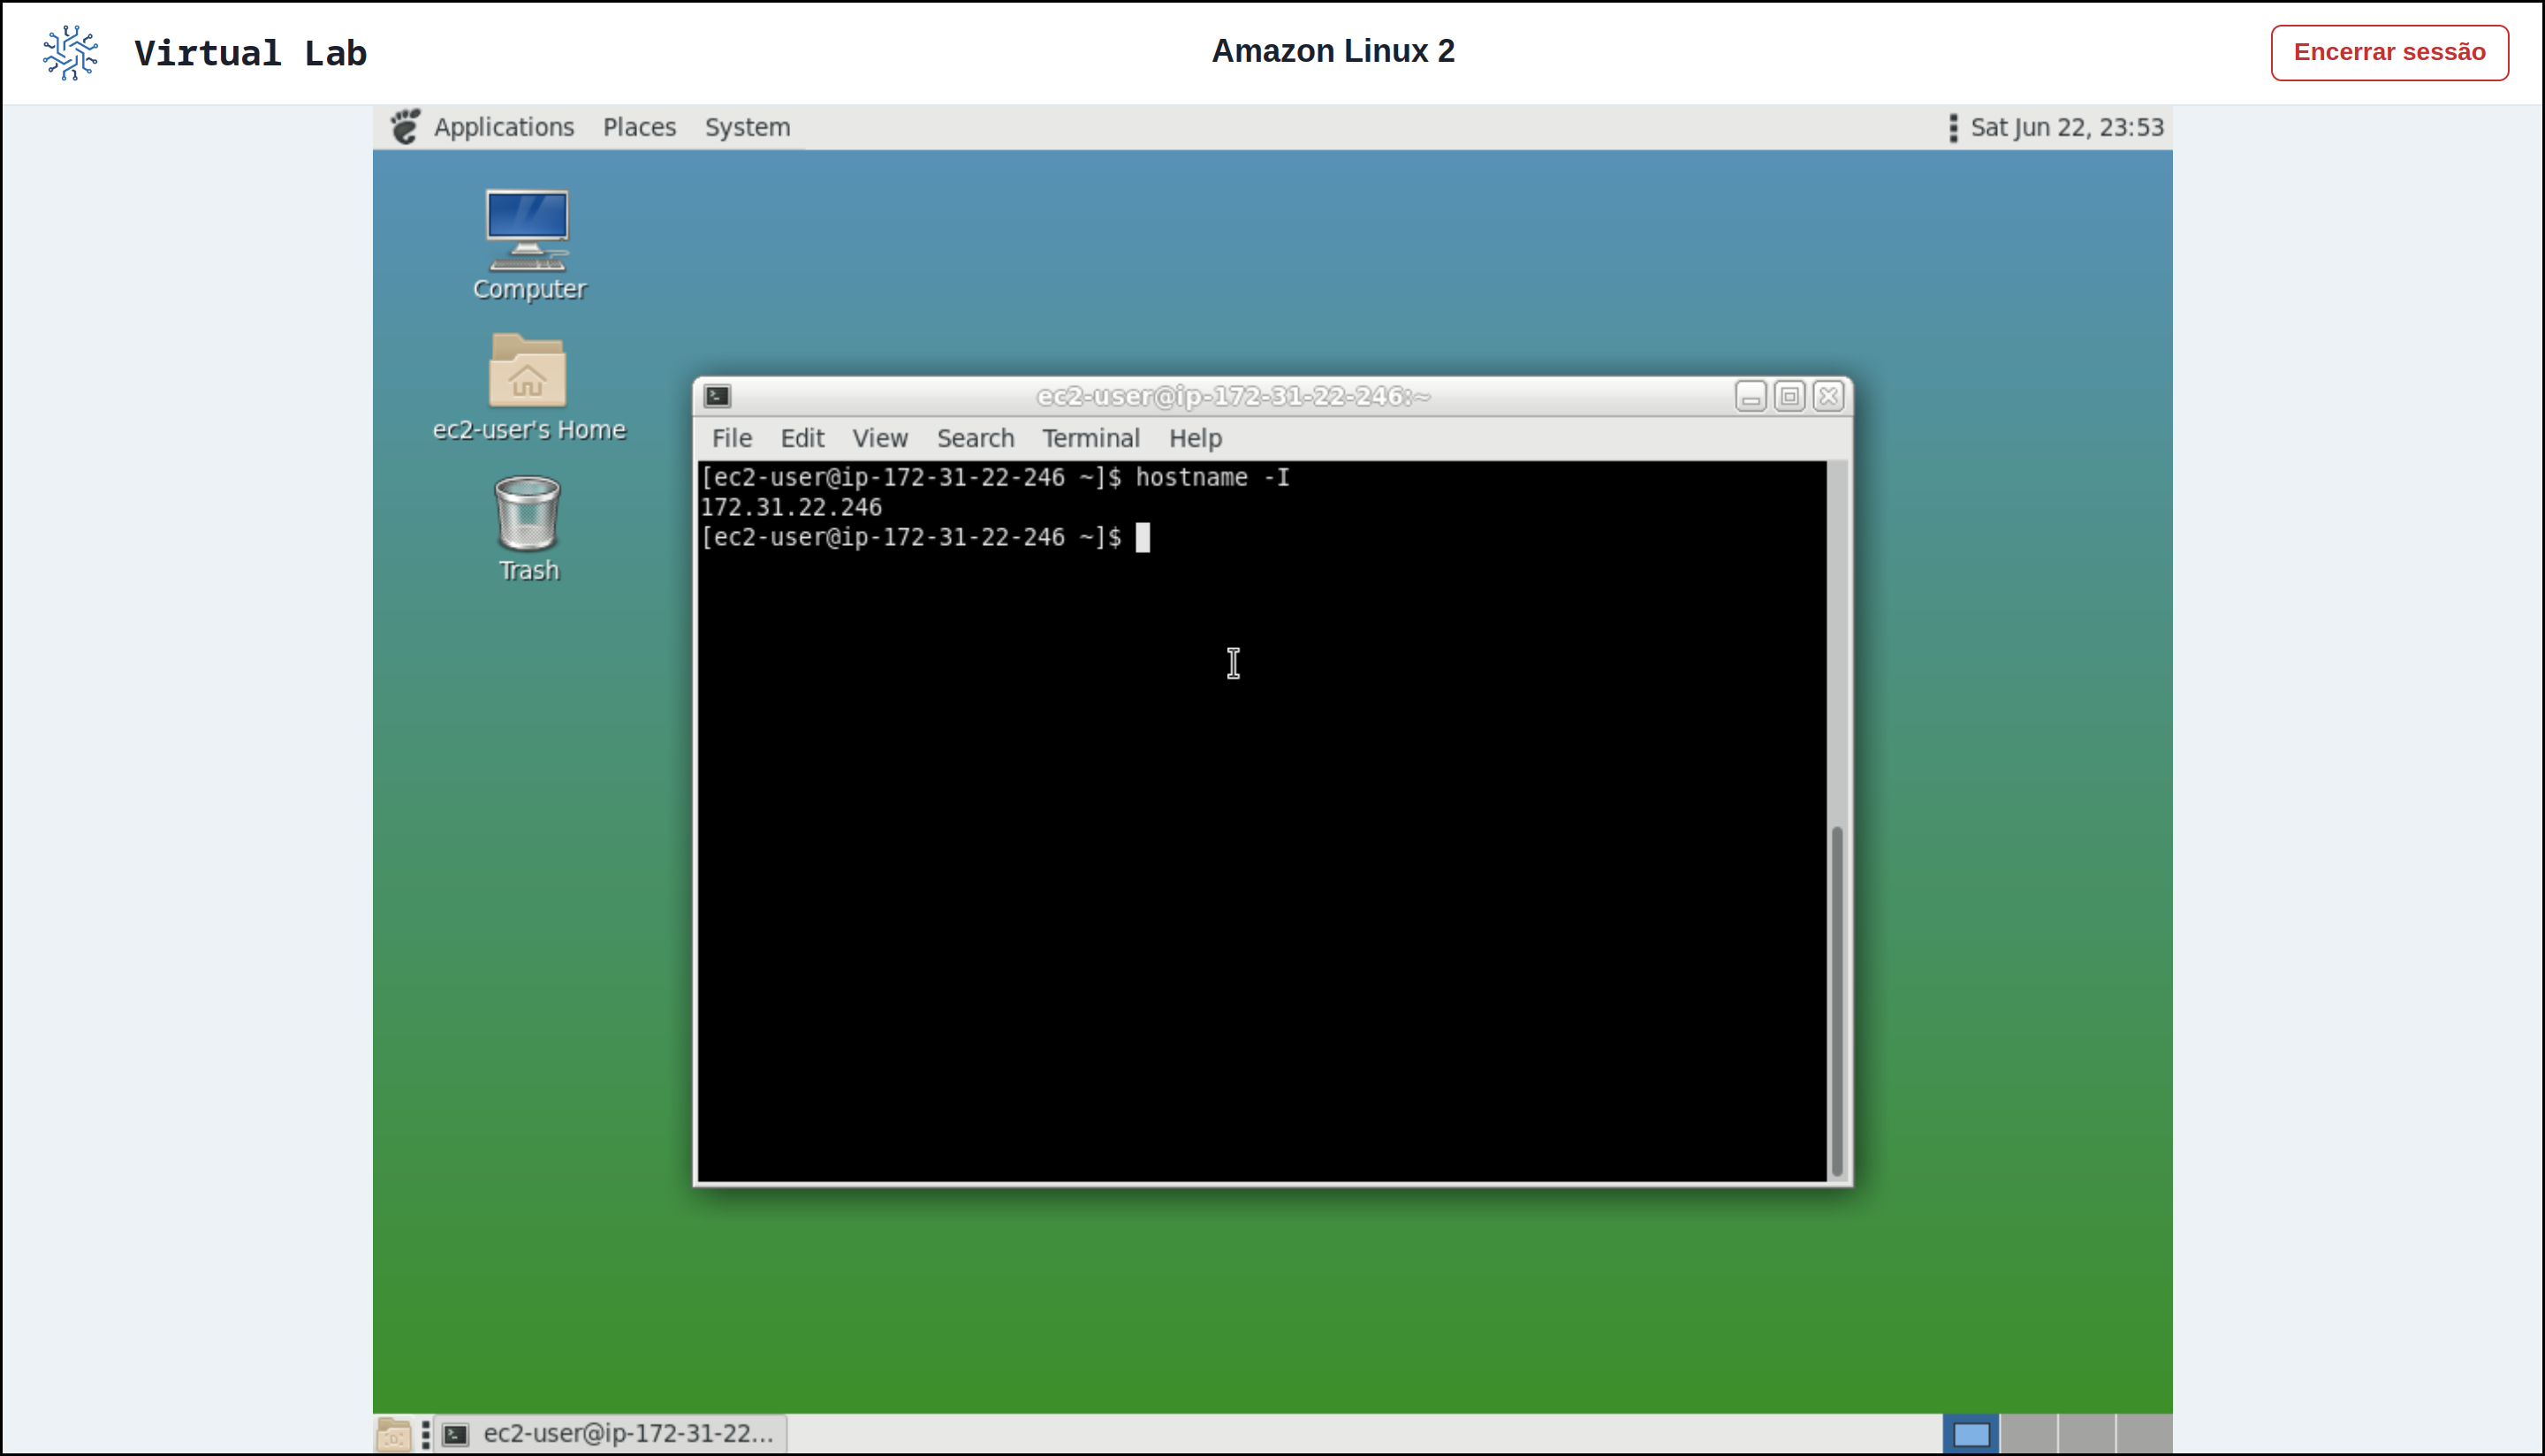
\includegraphics[width=\textwidth]{capitulos/3-resultados/files/connection.png}
\fonte{Autoria Própria (2024)}
\end{figure}


Novamente na página de listagem de instâncias, o usuário volta a visualizar os outros recursos disponíveis na interface. Para acessar suas informações pessoais, bem como suas cotas de uso do sistema, o usuário pode acionar o botão com seu nome de usuário no canto superior direito da tela, que apresenta os botões \texttt{Perfil} e \texttt{Sair}, como apresentado na \autoref{fig:userMenu} e então acionar o botão \texttt{Perfil} para ser redirecionado para a página de perfil do usuário, como apresentado na \autoref{fig:userProfile}.


\begin{figure}[H]
%\captionsetup{width=0.55\textwidth}%% Largura da legenda
\caption{Menu do usuário}
\label{fig:userMenu}
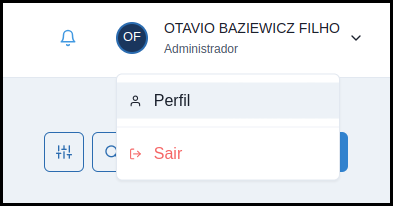
\includegraphics[width=\textwidth]{capitulos/3-resultados/files/user-menu.png}
\fonte{Autoria Própria (2024)}
\end{figure}

Na página de perfil do usuário o usuário pode visualizar suas informações pessoais, cotas de uso do sistema, bem como realizar a verificação de e-mail, que acontece através do envio de um e-mail de para o endereço cadastrado com um código que deve ser inserido no campo habilitado ao acionar o botão \texttt{Verificar Email}. É importante salientar que a verificação de e-mail é necessária para que o usuário possa recuperar a senha da conta, caso necessário. Por outro lado, essa funcionalidade não afeta usuários que utilizam o login integrado com o provedor de identidade externo.

\begin{figure}[H]
%\captionsetup{width=0.55\textwidth}%% Largura da legenda
\caption{Página de perfil do usuário}
\label{fig:userProfile}
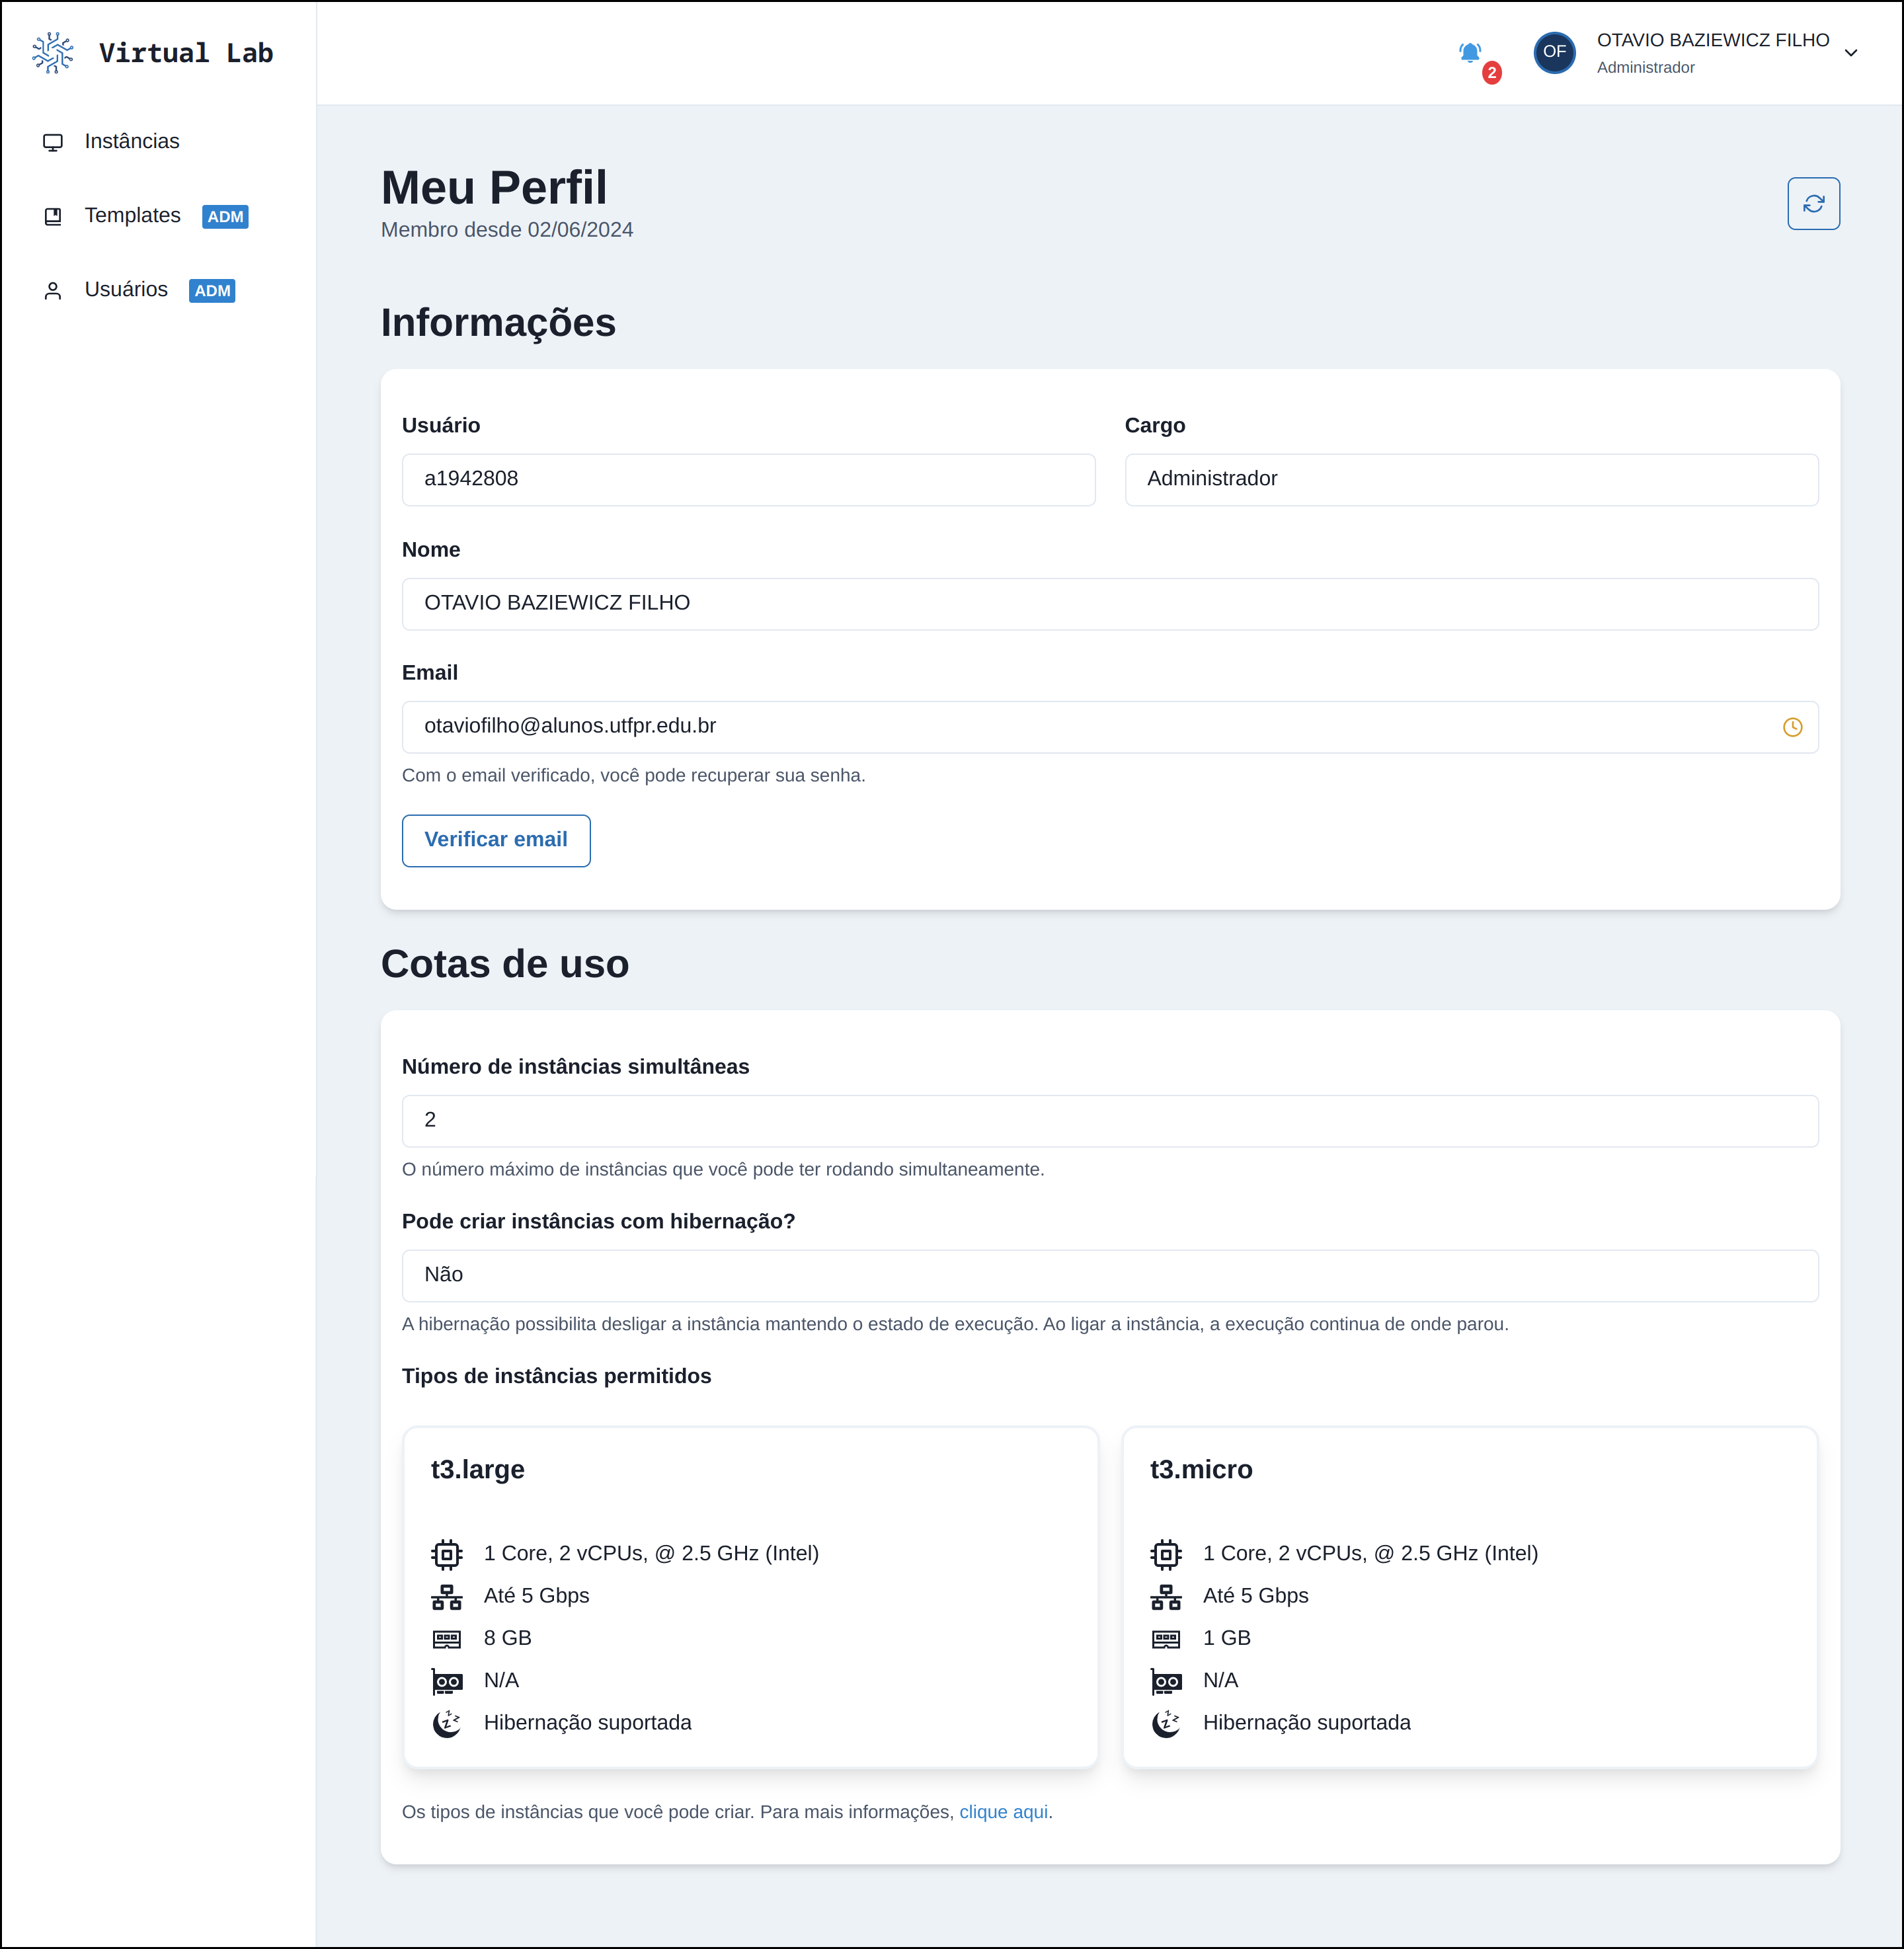
\includegraphics[width=\textwidth]{capitulos/3-resultados/files/profile.png}
\fonte{Autoria Própria (2024)}
\end{figure}

Usuários com o cargo de \gls{uadm} possuem a página de gerenciamento de templates, onde podem visualizar todos os templates de instancias disponíveis, bem como deletar templates existentes e criar novos templates a partir de imagens oficiais de sistemas operacionais. Essa página é acessível através do menu lateral, como apresentado na \autoref{fig:templatesPage}.

A listagem de templates é semelhante a listagem de instâncias, onde o usuário pode adaptar os filtros e utilizar a busca textual para encontrar templates específicos. Além disso, o usuário pode editar templates existentes, alterando o nome e a descrição, bem como excluir templates que não são mais necessários.

\begin{figure}[H]
%\captionsetup{width=0.55\textwidth}%% Largura da legenda
\caption{Página de templates de instâncias}
\label{fig:templatesPage}
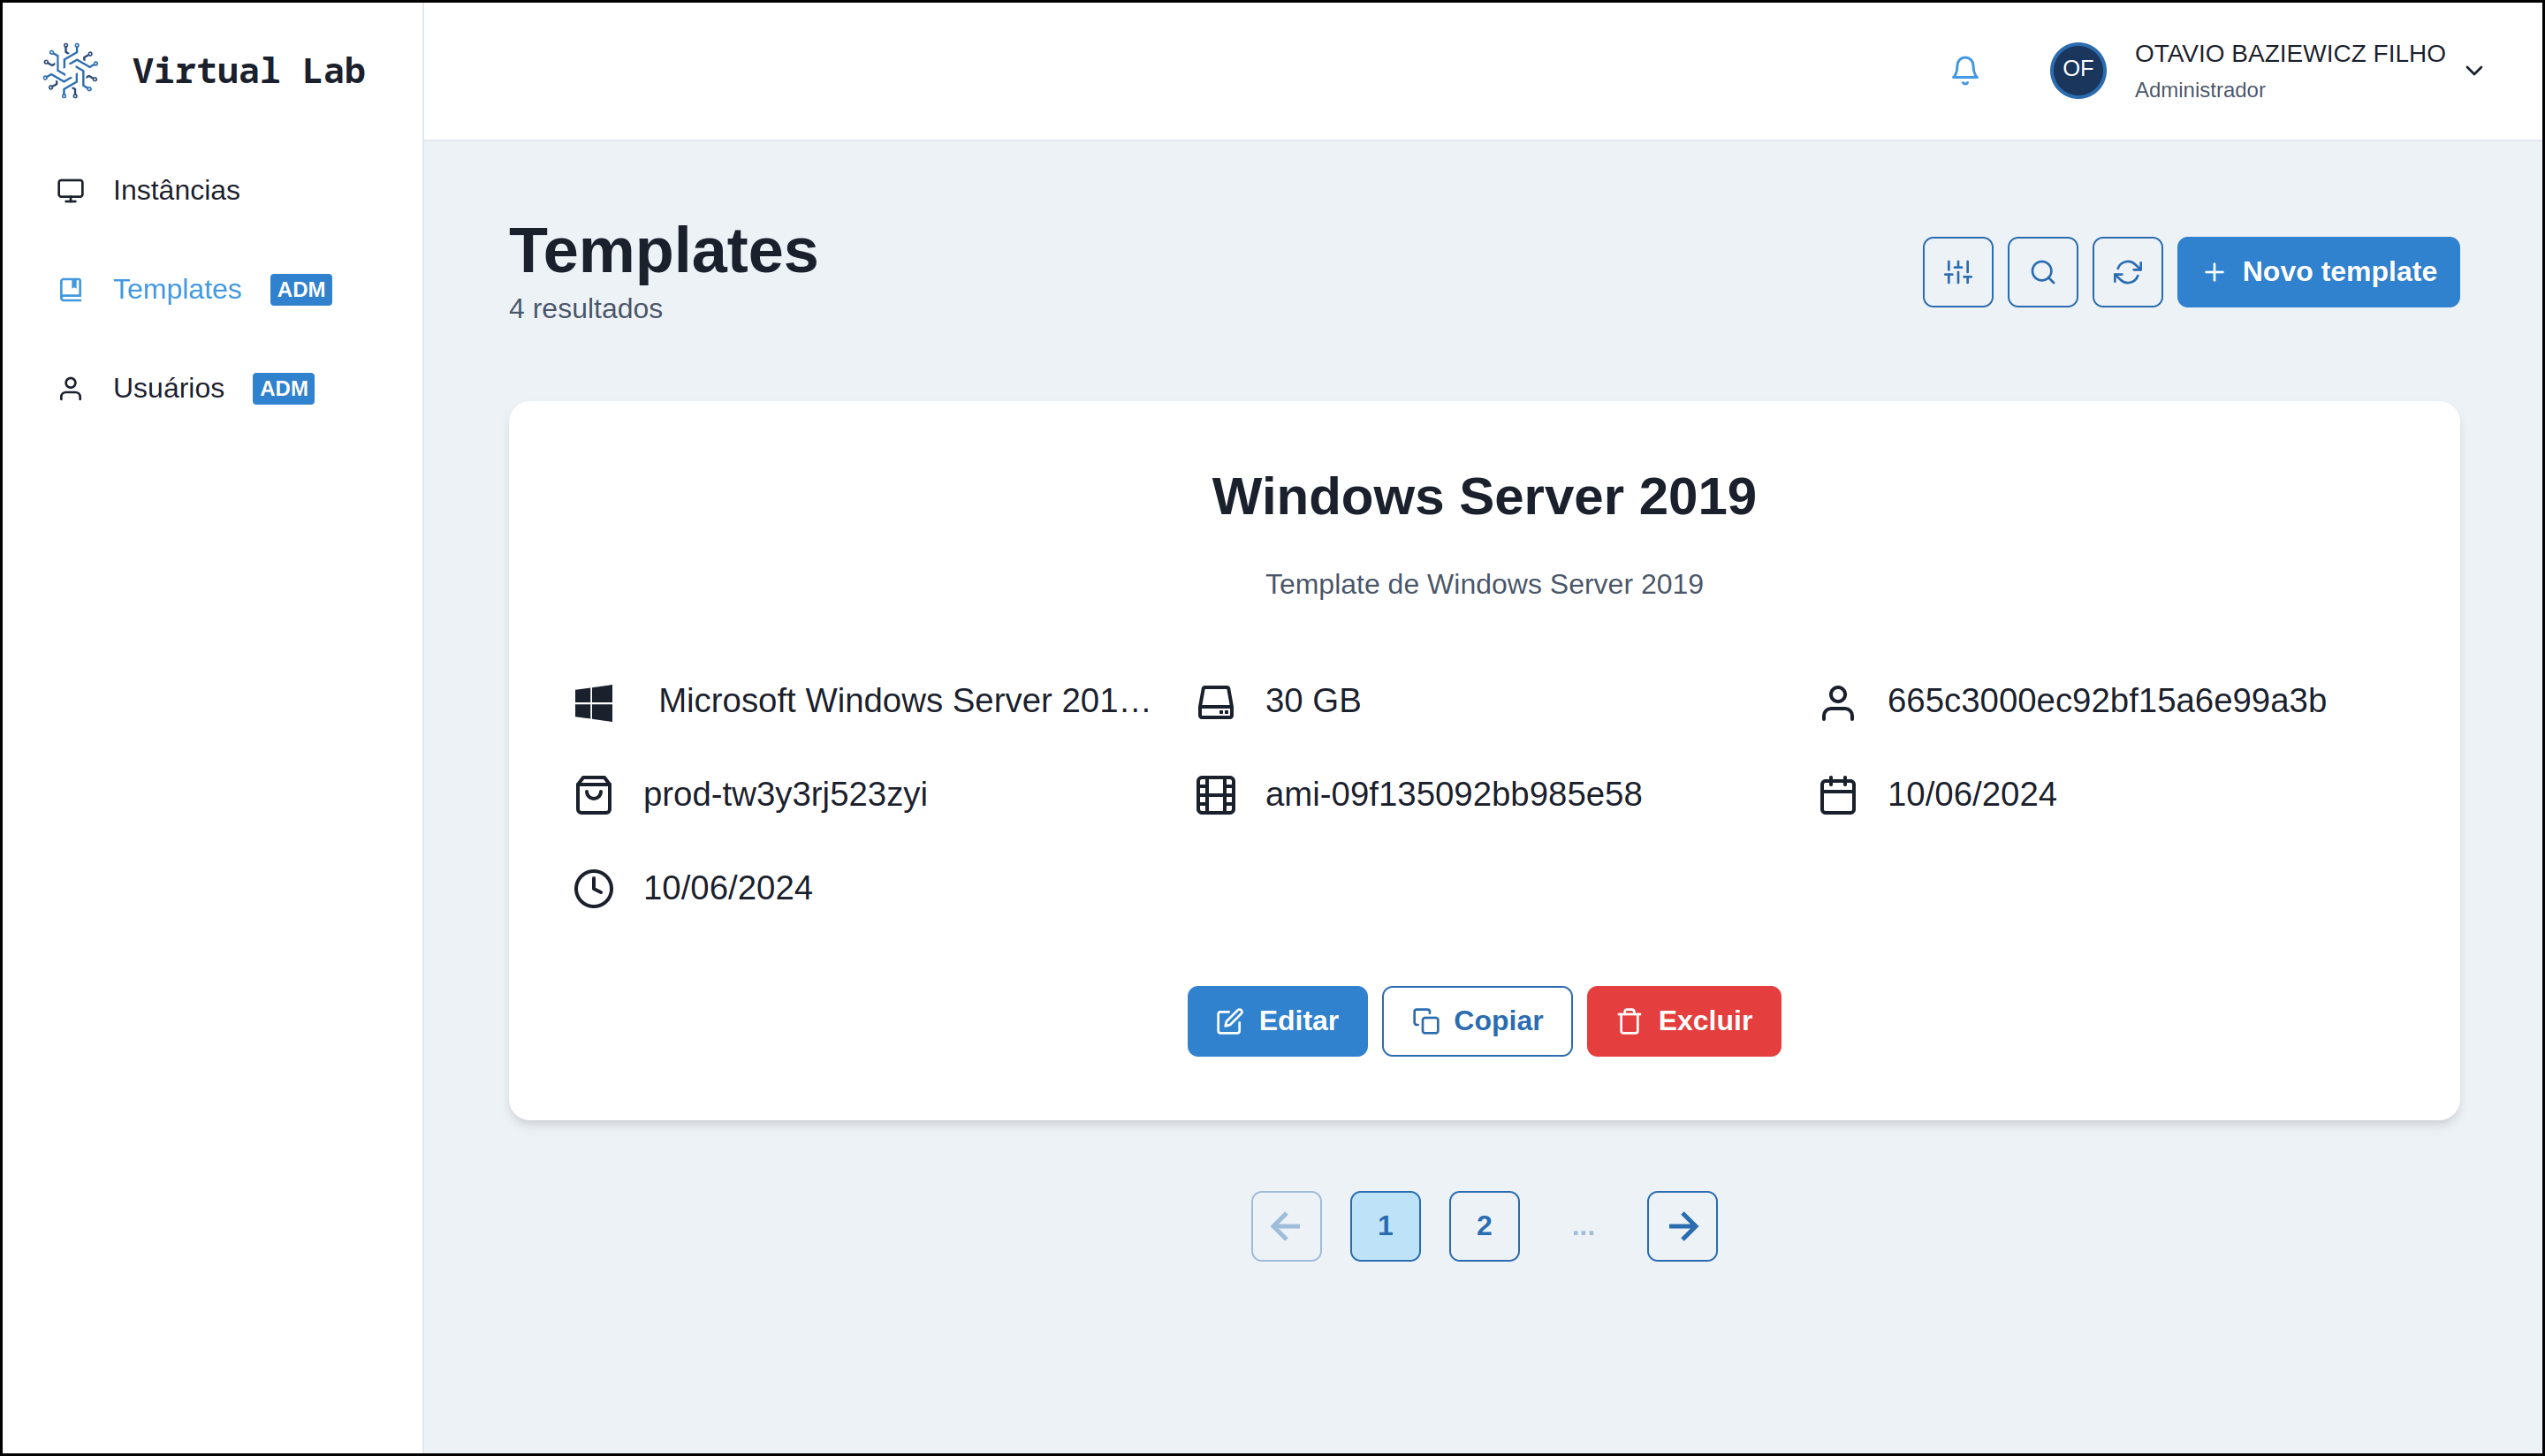
\includegraphics[width=\textwidth]{capitulos/3-resultados/files/templates.png}
\fonte{Autoria Própria (2024)}
\end{figure}

Ainda nessa página, quando o usuário aciona tanto o botão \texttt{Novo Template} quanto o botão \texttt{Copiar} de um template existente, o modal de criação de template é apresentado, como pode ser visto na \autoref{fig:createTemplate}. Nesse modal o usuário deve preencher os campos obrigatórios e escolher uma imagem de sistema operacional customizada ou recomendada pelo componente de escolha de imagem e em seguida acionar o botão \texttt{Criar Template} para confirmar a criação, que estará disponível disponível para todos os usuários com o cargo de \gls{ucom} ou \gls{uadm}. Diferente da criação de template a partir de uma instância existente, a criação de template a partir de uma imagem existente é instantâneo.

\begin{figure}[H]
%\captionsetup{width=0.55\textwidth}%% Largura da legenda
\caption{Modal de criação de template de instância}
\label{fig:createTemplate}
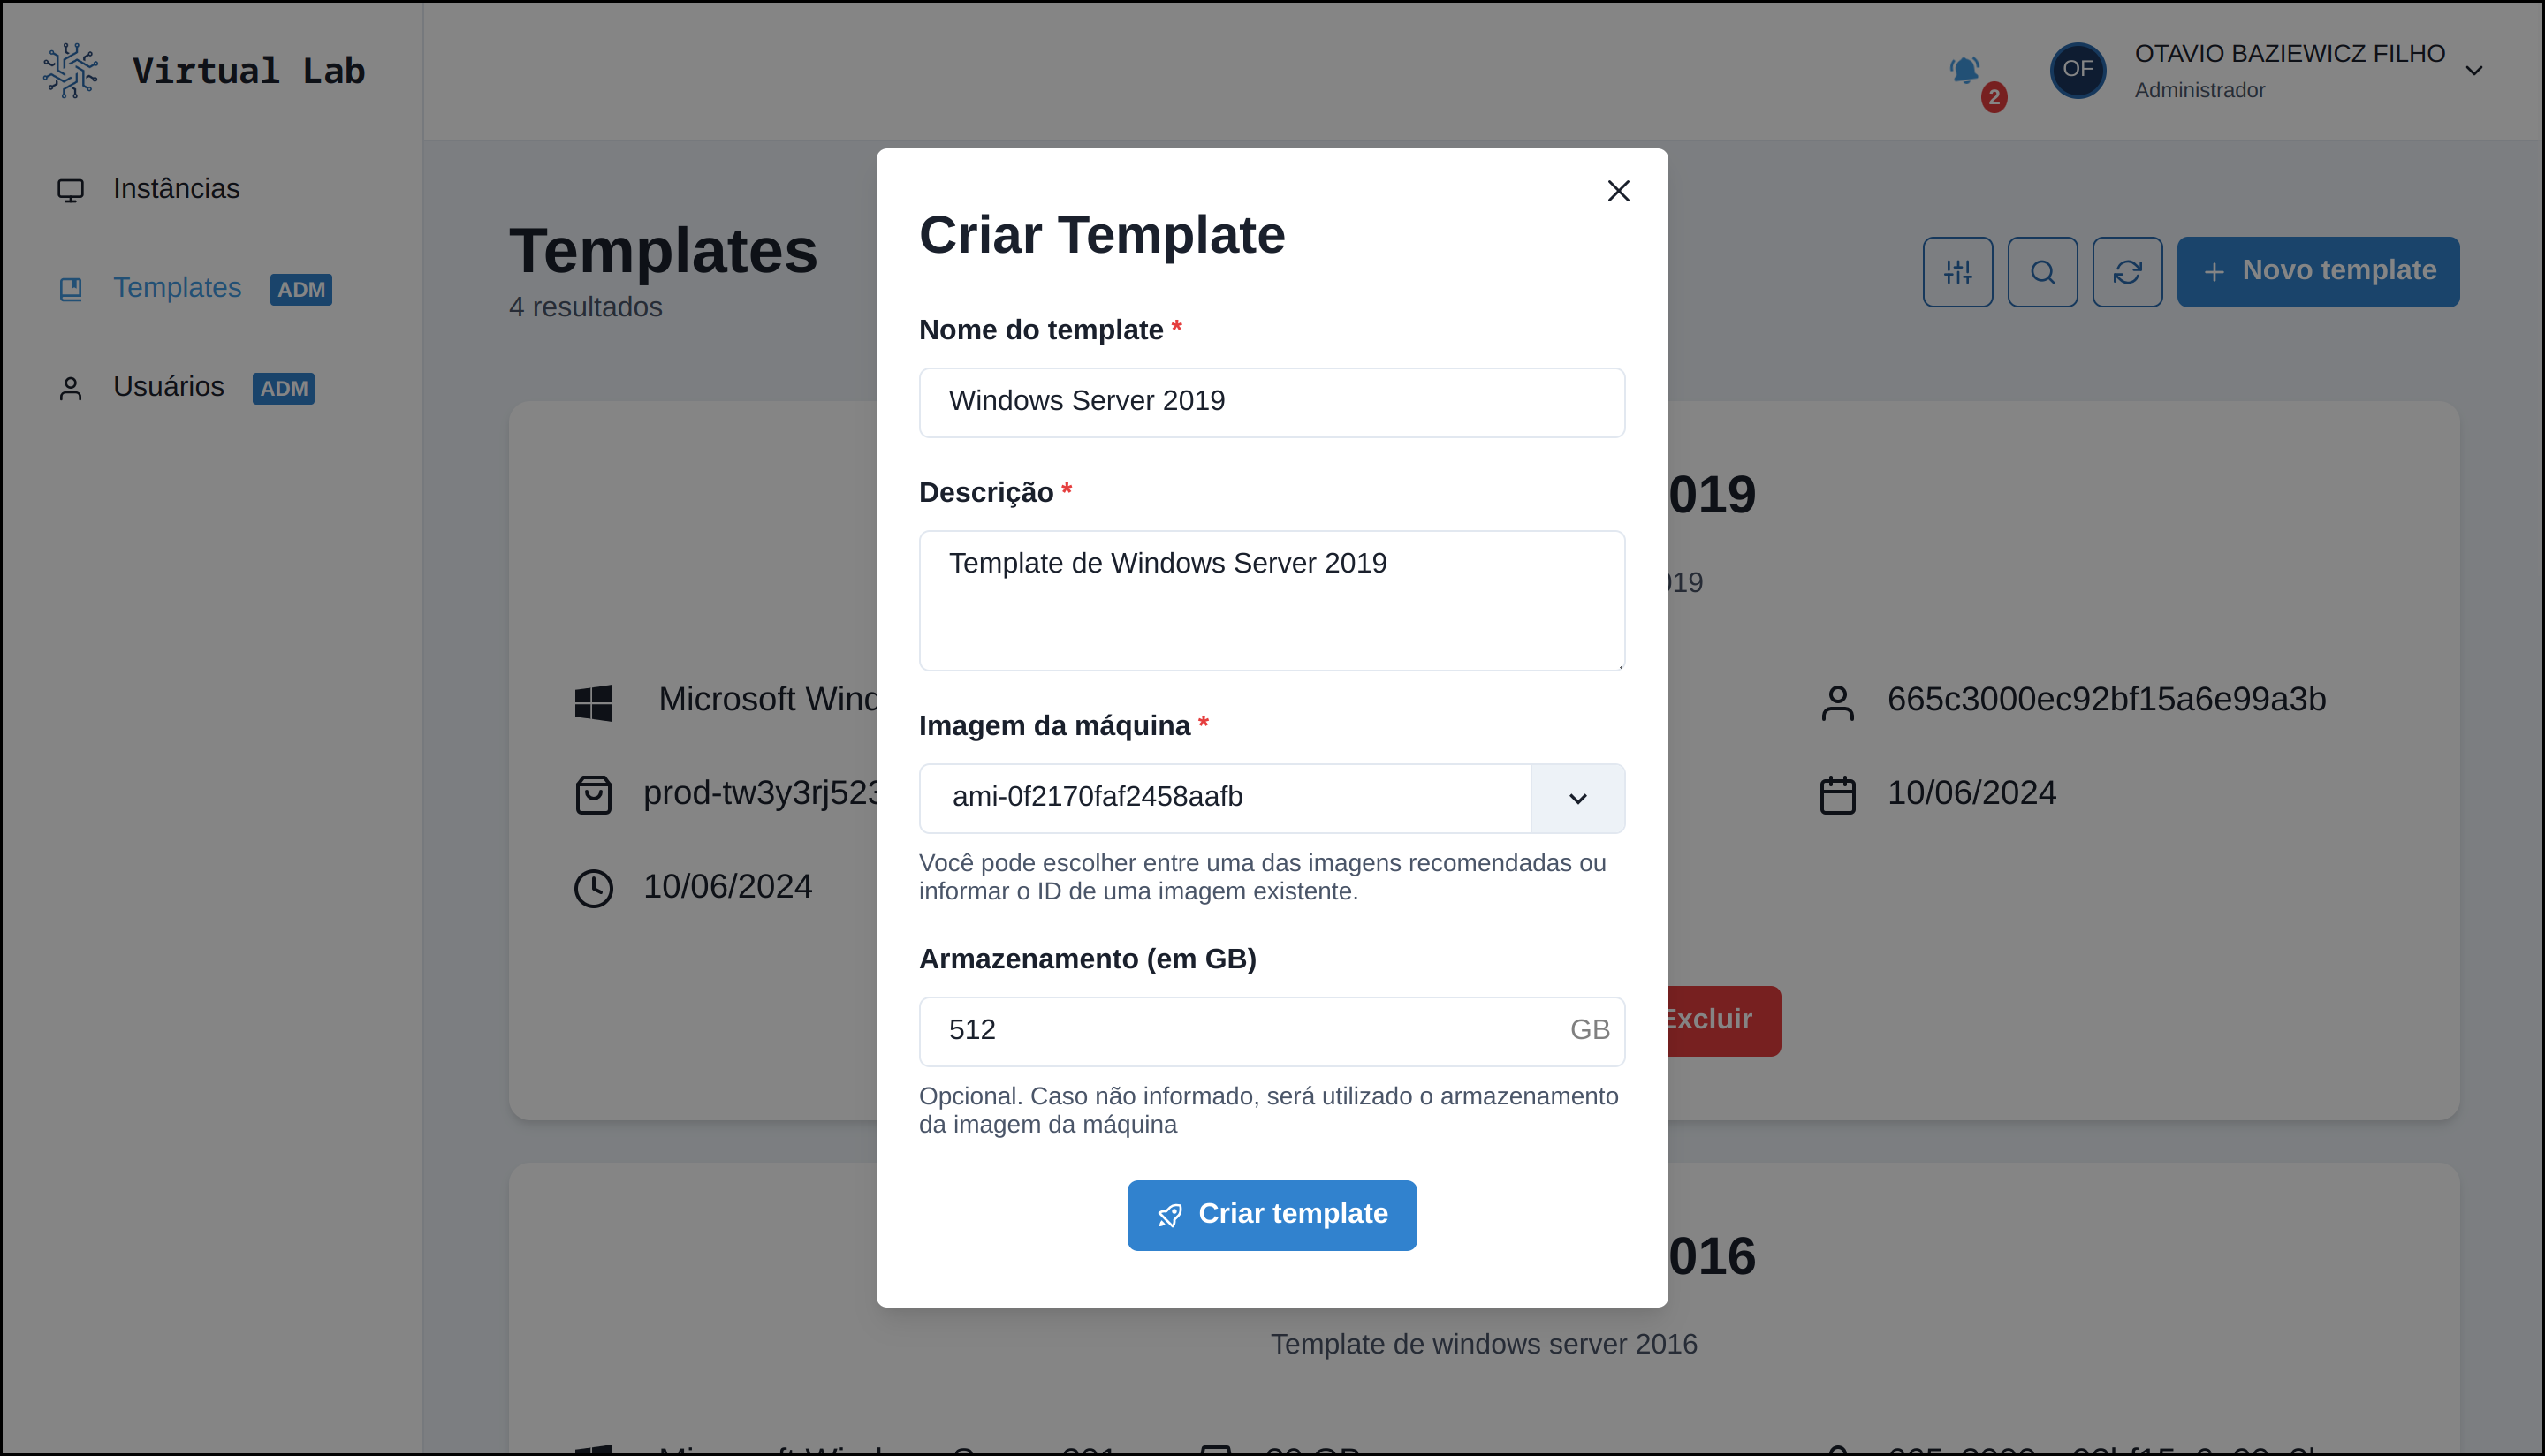
\includegraphics[width=\textwidth]{capitulos/3-resultados/files/create-template.png}
\fonte{Autoria Própria (2024)}
\end{figure}

Usuários com cargo de \gls{uadm} possuem ainda a página de gerenciamento de usuários, onde podem visualizar todos os usuários cadastrados no sistema, bom como aprovar usuários pendentes e atualizar as cotas de uso dos usuários. Essa página é acessível através do menu lateral, como apresentado na \autoref{fig:usersPage}. A listagem de usuários é semelhante a listagem de instâncias e templates, onde o usuário pode adaptar os filtros e utilizar a busca textual para encontrar usuários específicos, com a diferença que a apresentação dos usuários é feita através de uma tabela, onde cada linha representa um usuário e cada coluna uma informação do usuário.

\begin{figure}[H]
%\captionsetup{width=0.55\textwidth}%% Largura da legenda
\caption{Página de usuários}
\label{fig:usersPage}
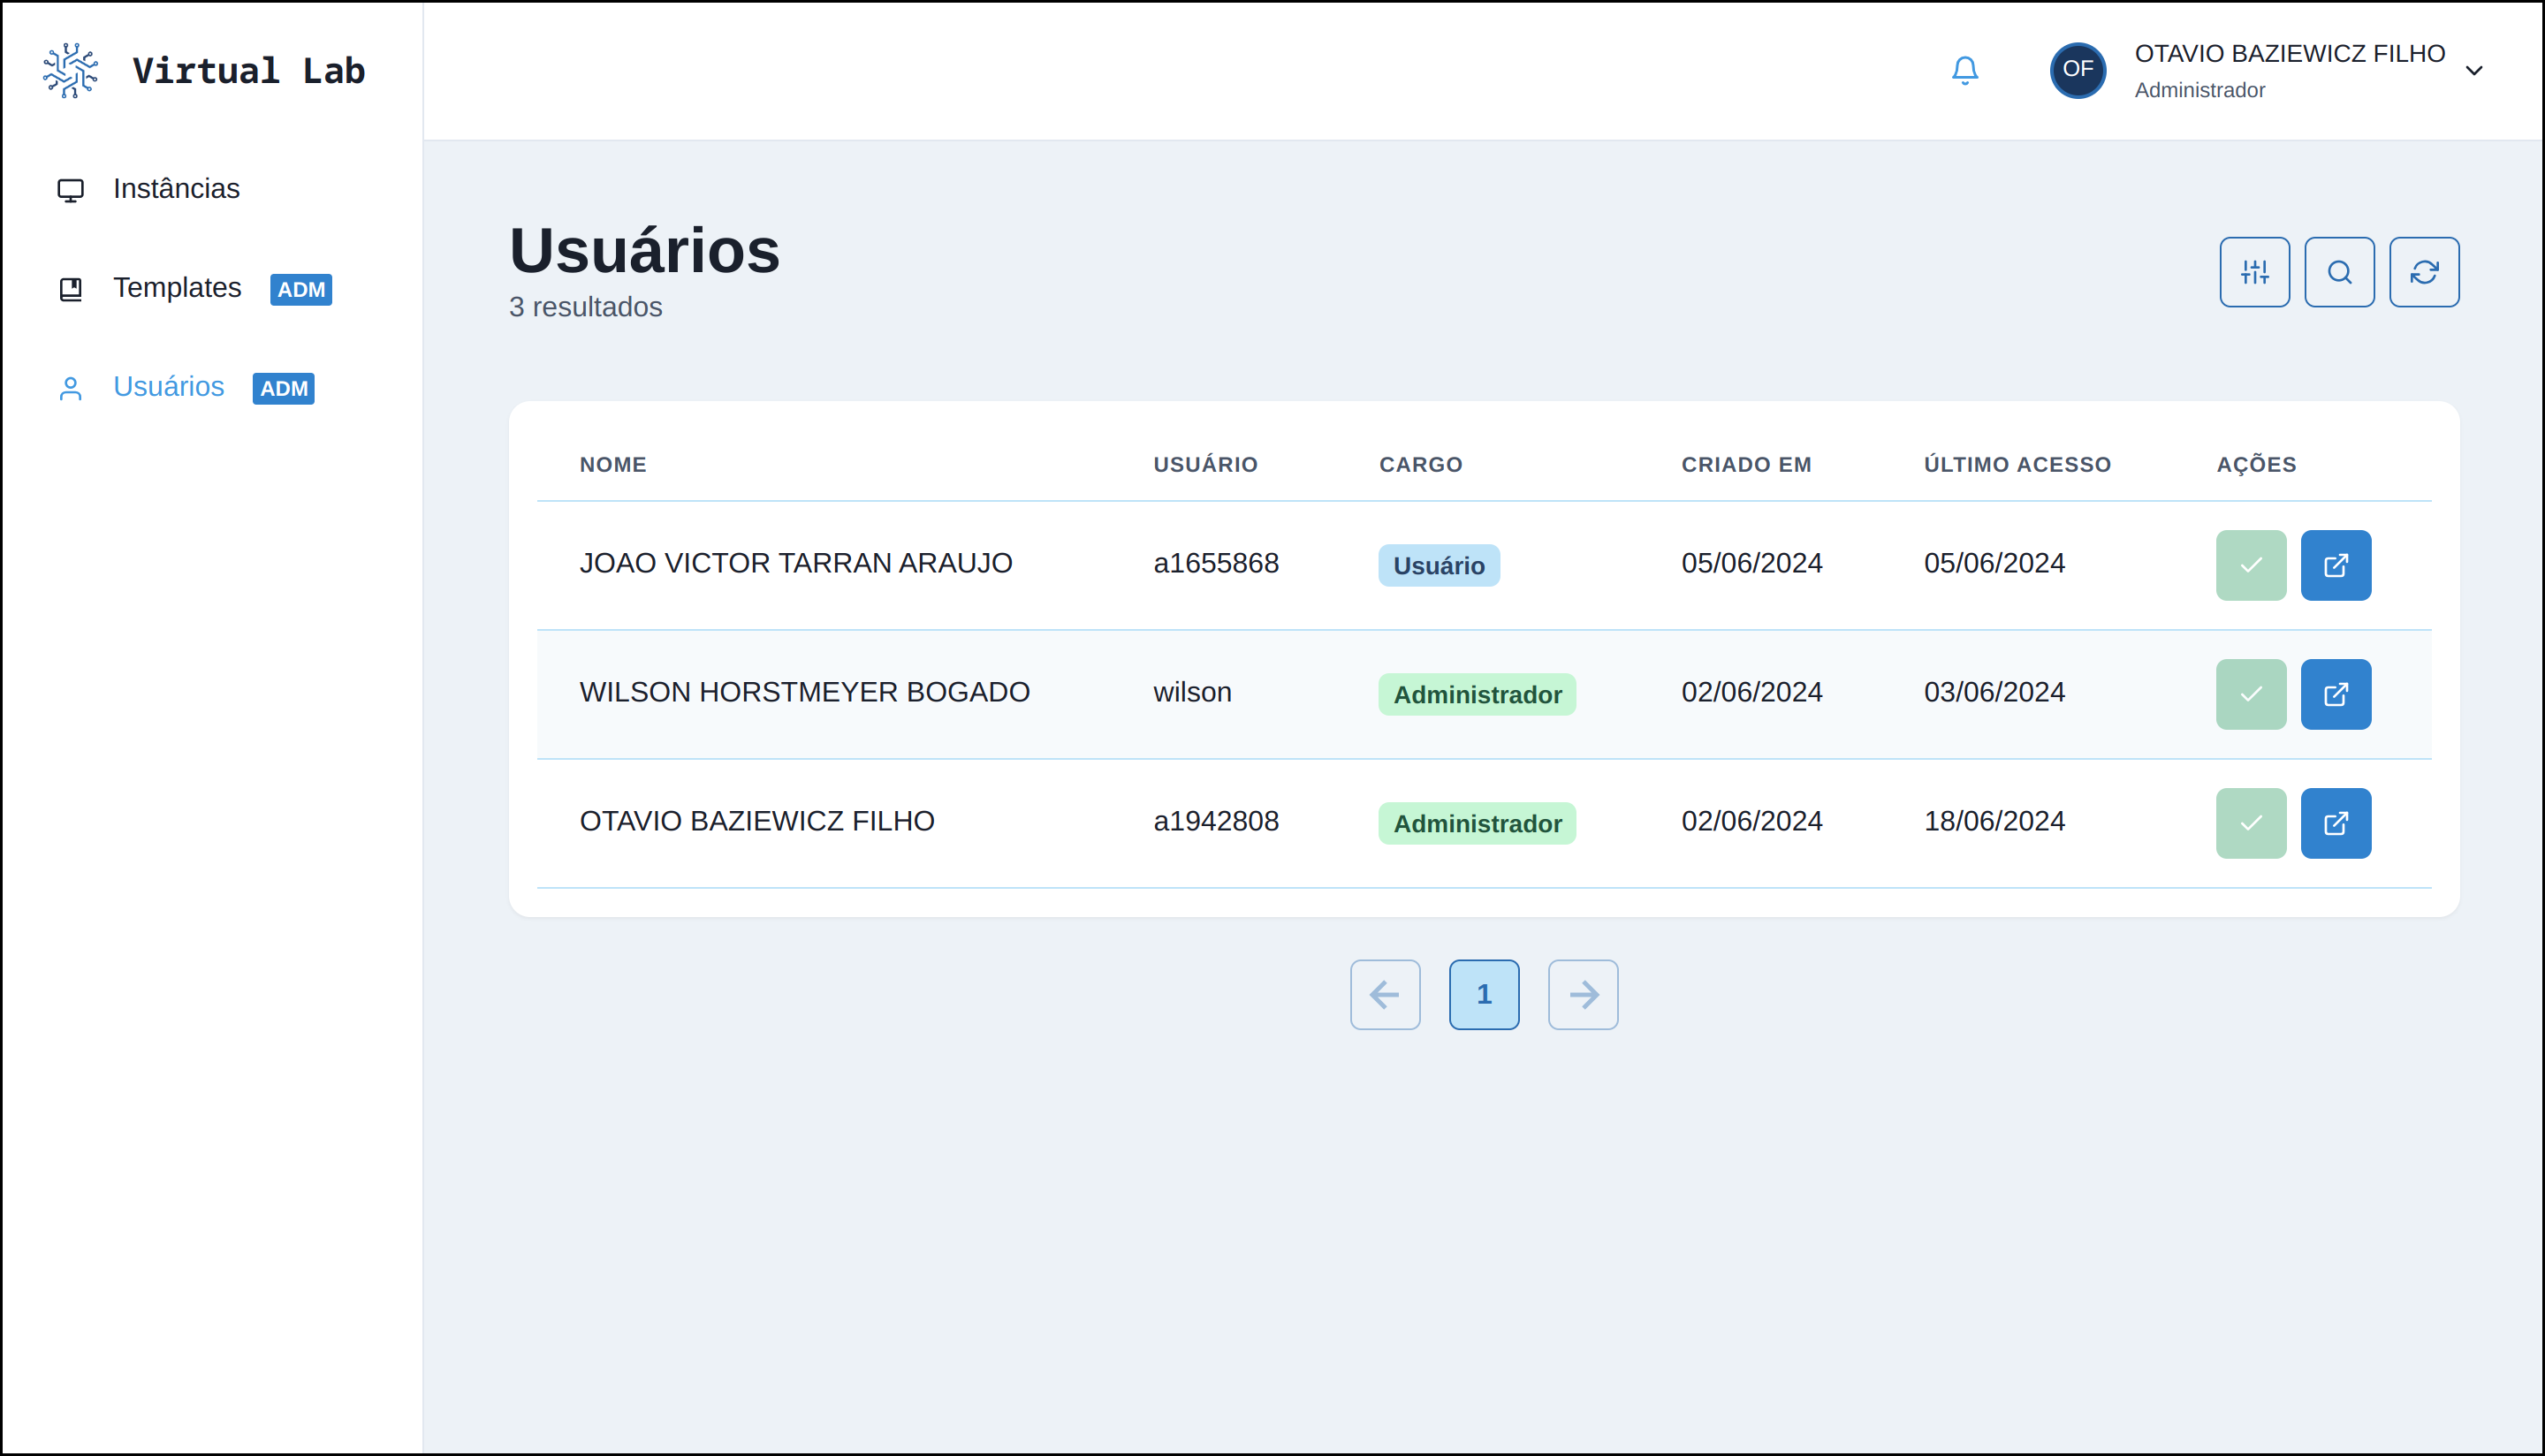
\includegraphics[width=\textwidth]{capitulos/3-resultados/files/users.png}
\fonte{Autoria Própria (2024)}
\end{figure}

Ao selecionar um usuário na listagem, agora na página de detalhes do usuário, é possível visualizar todas as informações do usuário, bem como atualizar o cargo do usuário e as cotas de uso do sistema. Essa página é apresentada na \autoref{fig:userDetails}.

\begin{figure}[H]
%\captionsetup{width=0.55\textwidth}%% Largura da legenda
\caption{Página de detalhes do usuário}
\label{fig:userDetails}
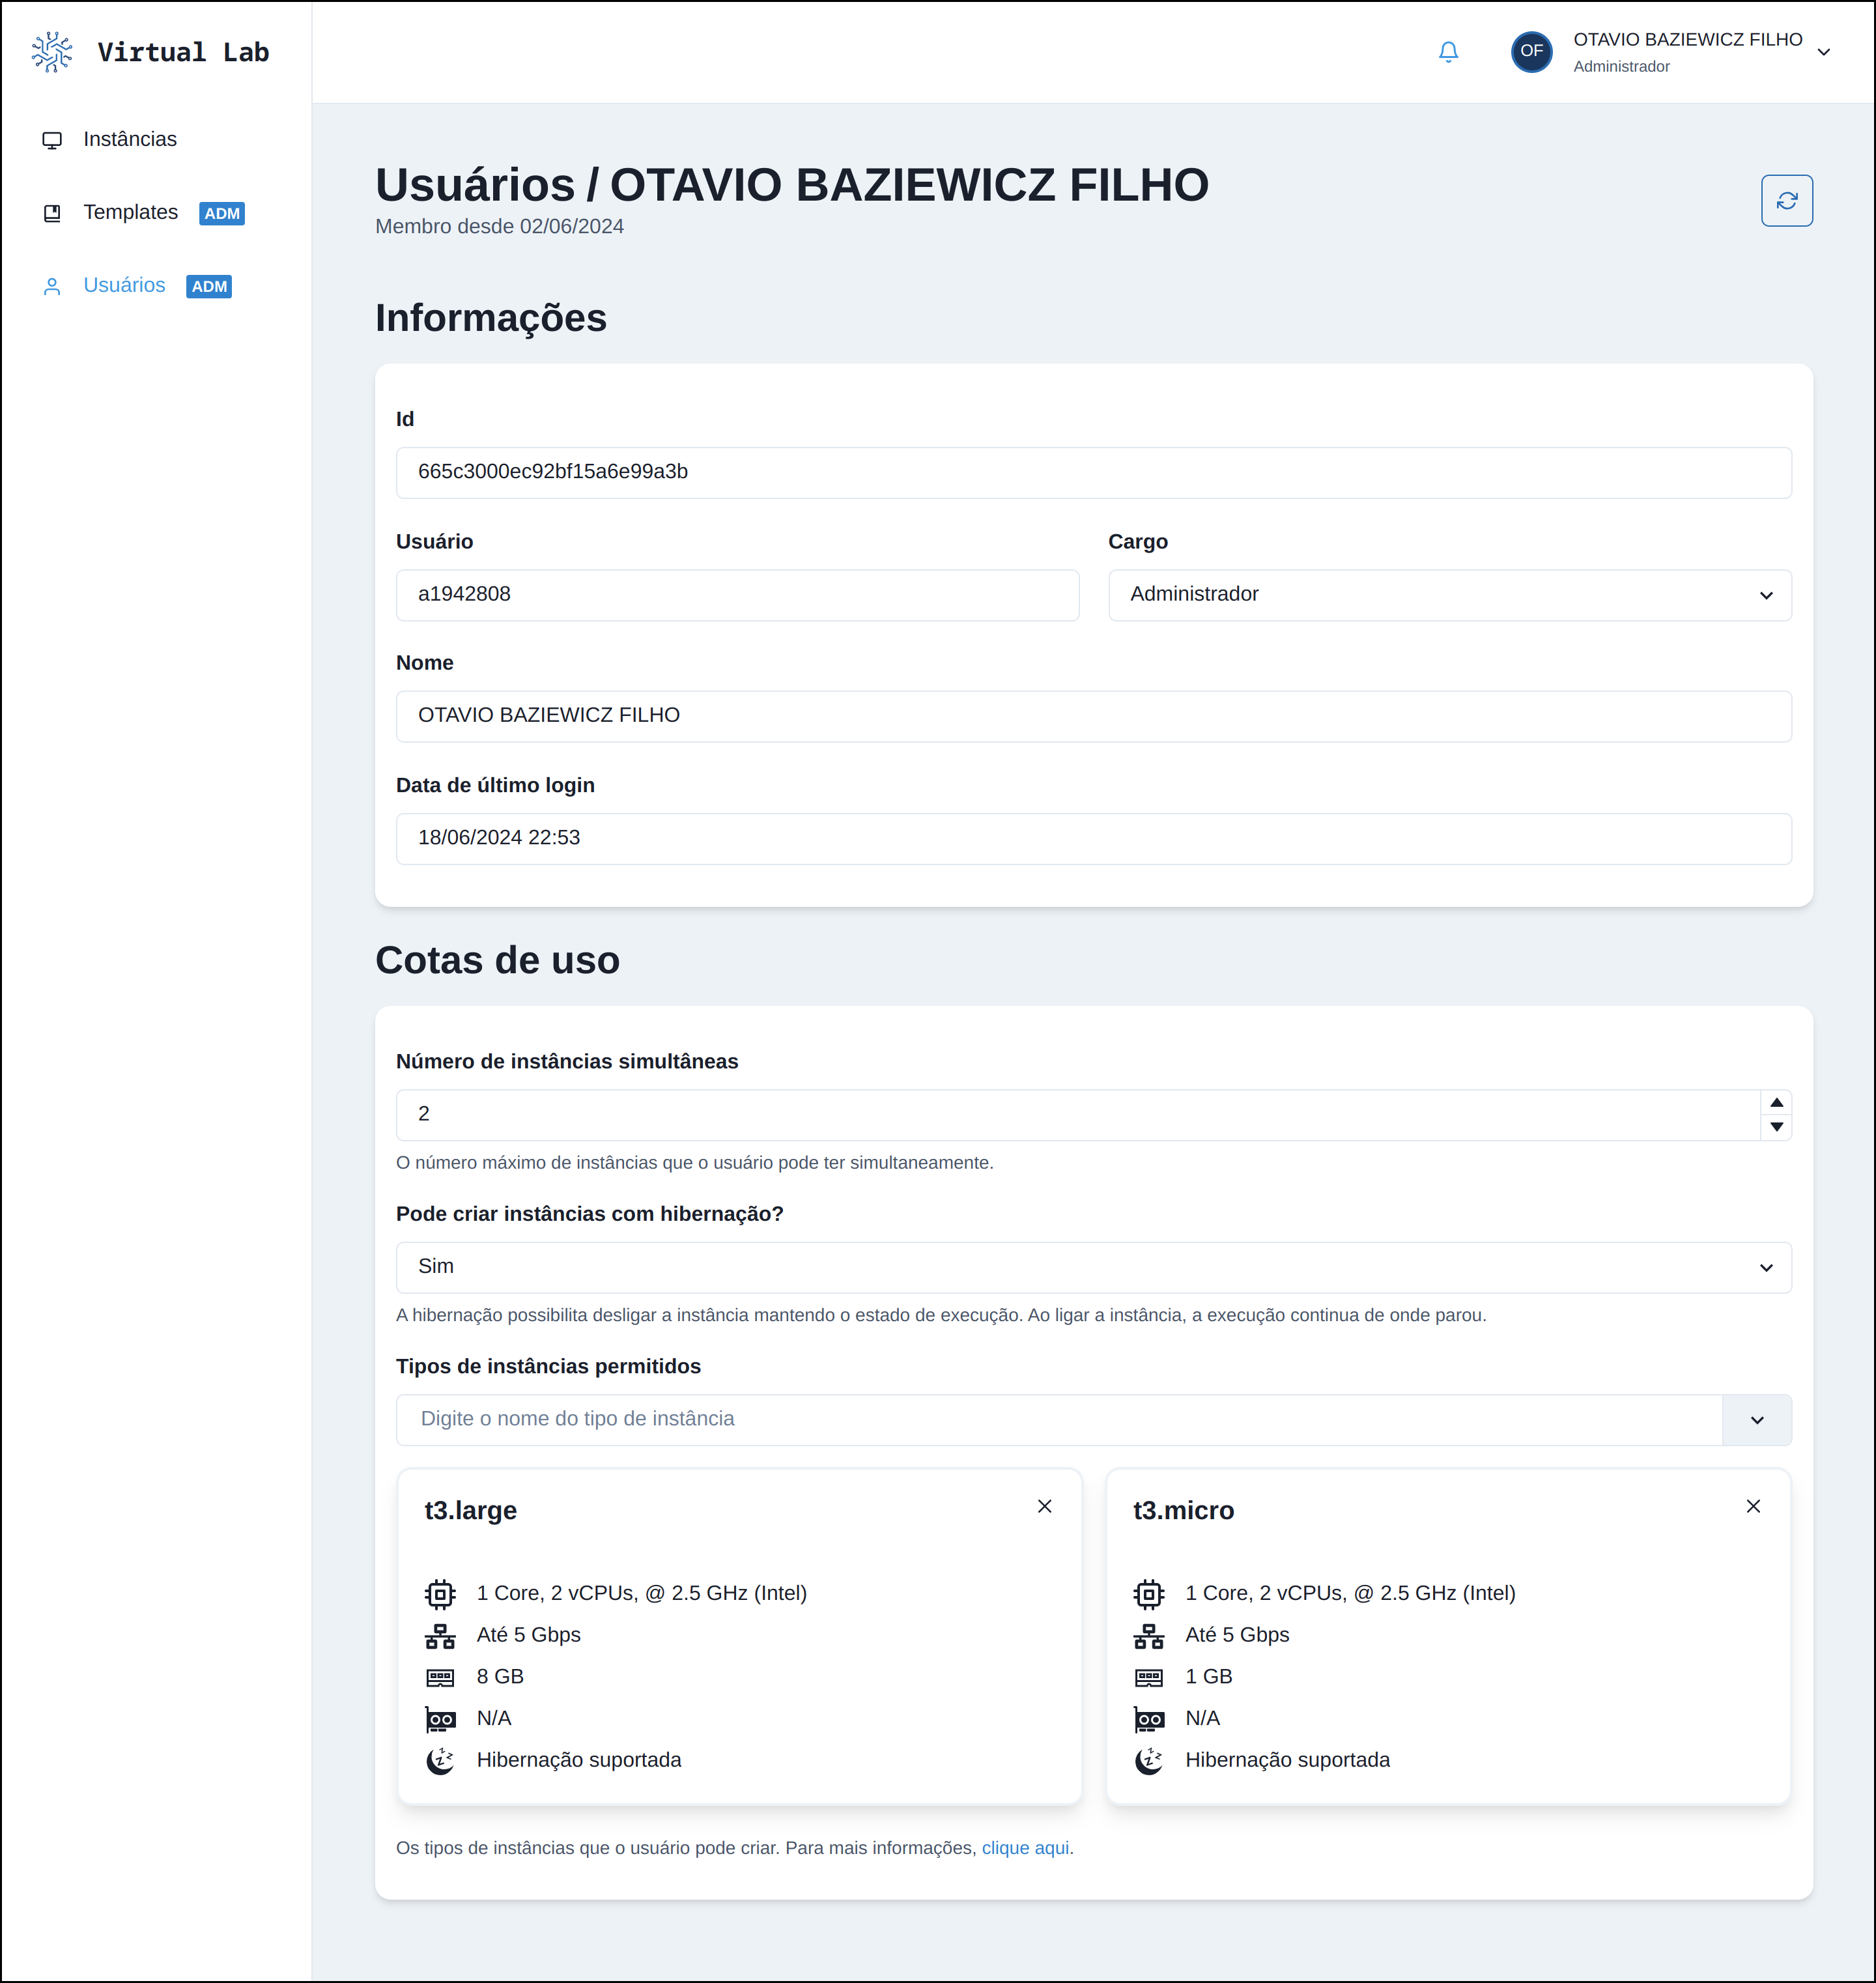
\includegraphics[width=\textwidth]{capitulos/3-resultados/files/user-page.png}
\fonte{Autoria Própria (2024)}
\end{figure}

\section{Estimativa de custos}
\label{sec:estimativaDeCustos}

Como parte do projeto, foi realizada uma estimativa de custos para a utilização do sistema em diferentes cenários de uso. A estimativa foi feita com base nos preços de mercado da \gls{aws} através da calculadora de preços disponível em seu site oficial. 

A primeira estimativa leva em consideração um cenário de uso onde 100 instâncias são utilizadas por 1 hora e 30 minutos por dia, durante 30 dias, com picos de utilização de 5 dias por semana. As instâncias são do tipo \texttt{t3.micro} com 2 vCPU e 1GB de memória RAM.

O custo total estimado para esse cenário é de U\$ 289.82/mês, ou R\$ 1.573,72/mês com a cotação do dólar a R\$ 5,43, como apresentado na \autoref{tab:costEstimation1}.


\begin{longtable}{@{\extracolsep{\fill}}l l}%% Ambiente longtable
\caption{Primeira estimativa de custos\label{tab:costEstimation1}} \\%% Legenda e rótulo
\toprule
\textbf{Serviço} & \textbf{Custo} \\
\midrule
\endfirsthead%% Encerra cabeçalho da primeira página
\caption[]{Primeira estimativa de custos} \\%% Legenda
\multicolumn{2}{r}{\textbf{(continuação)}} \\
\toprule
\textbf{Serviço} & \textbf{Custo} \\
% \midrule
\endhead%% Encerra cabeçalho das demais páginas
% \midrule
\multicolumn{2}{r}{\textbf{(continua)}} \\
\endfoot%% Encerra rodapé das demais páginas
% \bottomrule
\\[-0.5\linha]
\caption*{\nomefonte: Autoria própria (2024)} \\
\endlastfoot%% Encerra rodapé da última página

Amazon Cognito & R\$ 0.75 \\ \hline
S3 Standard & R\$ 0.12 \\ \hline
Data Transfer & R\$ 4.50 \\ \hline
AppSync API Request & R\$ 0.01 \\ \hline
Appsync Data Transfer & R\$ 0.90 \\ \hline
Amazon API Gateway & R\$ 1.00 \\ \hline
AWS Service Catalog & R\$ 0.35 \\ \hline
Standard topics & R\$ 0.00 \\ \hline
AWS Lambda & R\$ 5.83 \\ \hline
Application Load Balancer & R\$ 36.87 \\ \hline
Amazon Elastic Container Registry & R\$ 0.20 \\ \hline
Amazon EventBridge & R\$ 1.00 \\ \hline
AWS Fargate & R\$ 26.00 \\ \hline
Amazon EC2 & R\$ 212.29 \\ \hline

\end{longtable}

O segundo cenário de uso leva em consideração a utilização apenas dos serviços essenciais para manter o sistema funcionando. Essa estimativa visa entender o custo da infraestrutura em períodos de recesso, onde o sistema deve ficar sem acessos por aproximadamente 1 mês.

O custo total estimado para esse cenário é de U\$ 35.13/mês, ou R\$ 185,32/mês com a cotação do dólar a R\$ 5,43, como apresentado na \autoref{tab:costEstimation2}.

\begin{longtable}{@{\extracolsep{\fill}}l l}%% Ambiente longtable
\caption{Segunda estimativa de custos\label{tab:costEstimation2}} \\%% Legenda e rótulo
\toprule
\textbf{Serviço} & \textbf{Custo} \\
\midrule
\endfirsthead%% Encerra cabeçalho da primeira página
\caption[]{Segunda estimativa de custos} \\%% Legenda
\multicolumn{2}{r}{\textbf{(continuação)}} \\
\toprule
\textbf{Serviço} & \textbf{Custo} \\
% \midrule
\endhead%% Encerra cabeçalho das demais páginas
% \midrule
\multicolumn{2}{r}{\textbf{(continua)}} \\
\endfoot%% Encerra rodapé das demais páginas
% \bottomrule
\\[-0.5\linha]
\caption*{\nomefonte: Autoria própria (2024)} \\
\endlastfoot%% Encerra rodapé da última página

Amazon Cognito & R\$ 0.00 \\ \hline
S3 Standard & R\$ 0.12 \\ \hline
Data Transfer & R\$ 4.50 \\ \hline
AppSync API Request & R\$ 0.00 \\ \hline
Appsync Data Transfer & R\$ 0.00 \\ \hline
Amazon API Gateway & R\$ 0.00 \\ \hline
AWS Service Catalog & R\$ 0.00 \\ \hline
Standard topics & R\$ 0.00 \\ \hline
AWS Lambda & R\$ 0.00 \\ \hline
Application Load Balancer & R\$ 16.43 \\ \hline
Amazon Elastic Container Registry & R\$ 0.20 \\ \hline
Amazon EventBridge & R\$ 0.00 \\ \hline
AWS Fargate & R\$ 13.88 \\ \hline
Amazon EC2 & R\$ 0.00 \\ \hline

\end{longtable}

A comparação de custos em dois cenários distintos de uso do sistema, onde um cenário representa um uso com picos diários e o outro um uso mínimo, permite que a instituição de ensino tenha uma visão mais clara dos custos envolvidos na utilização do sistema e possa planejar a utilização do sistema de acordo com suas necessidades e orçamento disponível.

Um ponto observado durante a estimativa de custos é que os serviços de infraestrutura que representam a maior parte dos custos quando o sistema está em sua capacidade mínima de utilização são os serviços que servem de base para o funcionamento do Gateway de Conexão. Por outro lado, quando o sistema está em sua capacidade máxima de utilização, os serviços de infraestrutura representam uma parcela menor dos custos totais, com os serviços de instâncias \gls{ec2} representando a maior parte dos custos.